% ----------------------------- CONCETTI INTERMEDI -----------------------------------

\chapter{Concetti Intermedi}

%Possibili argomenti aggiuntivi di questo capitolo: 

% Map, Set, HashTable, Pair

% #include type_traits

%TODO: decltype.

% Random numbers? O nel beginner?
% std::chrono?

%TODO: inline functions.

%TODO: NULL (o null) vs nullptr

%TODO: explicit keyword, converting constructor.

%TODO: Private Destructor.

%TODO: copy elision.

%TODO: pure virtual destructors.

%TODO: typeid. type_traits

%TODO: SFINAE (Substitution Failure is Not An Error).

%TODO: cos'è la STL (Standard Template Library), questo dopo l'introduzione. (stl è un termine un po' vecchio).

%TODO: #include <bits/stdc++.h> è un header file che include tutti gli header files della STL. Non dovrebbe essere usato perché è lazy ed è un header del GCC che quindi potrebbe non andare in altri e non sai cosa fa perché i suoi contenuti non sono standard e ogni header file dovrebbe essere parsato il che renderebbe il tutto lento.

% -------------------------- SECTION: INTRODUZIONE -----------------------------------

\section{Introduzione}

\textsf{\small In questo capitolo, tratterò argomenti non necessariamente più complicati, ma che non considererei basi. } \\

\textsf{\small In questo capitolo vedremo ulteriori concetti riguardo le classi, il polimorfismo, le varie tipologie di costruttori, la programmazione generale, le lambdas, la programmazione funzionale e molto altro ancora..} \break

% -------------------------- SECTION: STL --------------------------------------------

\section{STL | Standard Template Library}

%TODO: cos'è e a cosa serve.

\subsection{Che cos'è \#include <bits/stdc++.h>?}

%TODO: #include <bits/stdc++.h> è un header file che include tutti gli header files della STL. Non dovrebbe essere usato perché è lazy ed è un header del GCC che quindi potrebbe non andare in altri e non sai cosa fa perché i suoi contenuti non sono standard e ogni header file dovrebbe essere parsato il che renderebbe il tutto lento.

% rende il codice non portabile.

% -------------------------- SECTION: TEMPLATES --------------------------------------

\newpage

\section{Templates}

\textsf{\small Immaginiamo di avere un codice, esempio questo:} \\

\begin{lstlisting}
	const int& max(const int& a, const int& b)
	{
		return a > b ? a : b;
	}
\end{lstlisting}

\textsf{\small Però ora se noi volessimo utilizzare questa funzione per i double, dovremmo copiarla e cambiare la tipologia da int a double.} \\

\begin{lstlisting}
	const int& max(const int& a, const int& b)
	{
		return a > b ? a : b;
	}

	const double& max(const double& a, const double& b)
	{
		return a > b ? a : b;
	}
\end{lstlisting}

\textsf{\small C'è un problema, se ora volessimo usare la stessa funzione, ma con i float? o con i char? Certo potremmo fare dei casts, ma così perderemmo dei dati, ma sopratutto ripeteremmo lo stesso codice più e più volte semplicemente per avere la stessa identica funzione, ma per tipologie diverse.} \\

\textsf{\small Inoltre, fare questo, continuare a ripetere lo stesso codice, violerebbe un'importante principio in programmazione, ovvero \textbf{DRY}: \emph{Don't repeat yourself}, in italiano, non ripeterti.} \break 

\textsf{\small Vogliamo cercare di ripetere lo stesso codice \textbf{il meno possibile} e \textbf{cercare di riutilizzare} codice che già abbiamo per altre funzionalità.} \\

\textsf{\small Quindi, c'è un modo migliore? Possiamo evitare di ripetere di scrivere lo stesso codice più e più volte? Si e Si! E facciamo questo attraverso i \textbf{templates}!} \break

\textsf{\small \textbf{Definizione:} I \textbf{templates} sono la fondazione della programmazione generale che riguarda lo scrivere codice che è indipendente dalla tipologia. } \\

\textsf{\small Quindi un \textbf{template} ti permette di creare uno stampino che funziona con qualsiasi tipo di variabile.} \\

\textsf{\small Come facciamo a dire al compilatore che vogliamo usare una variabile generica? Usiamo \textbf{typename} per dire che l'identificatore che segue è una tipologia e lo mettiamo all'interno del "diamantino", ovvero <>.} \\

\textsf{\small }

\begin{lstlisting}
	template <tipologia> tipoDiRitorno nomeDellaFunzione(lista dei parametri)
	{
		// corpo della funzione.
	}

	// Quindi usiamo una tipologia generica e la indichiamo con T, ma avremmo potuto usare qualsiasi altra lettera.
	template<typename T>
	const T& max(const T& a, const T& b)
	{
		return a > b ? a : b;
	}

	int x = 5, y = 3;
	std::cout << "Max tra due int: " << max(a, b) << std::endl; // Output: Max tra due int: 5
	
	double d1 = 3.69, d2 = 7.89;
	std::cout << "Max tra due double: " << max(a, b) << std::endl; // Output: Max tra due double: 7.89
	
	// Fate attenzione che se state usando 'using namespace std', avrete due funzioni chiamate max, una della libreria standard e l'altra questa in questo esempio.
	// In quel caso vi conviene rinominare la vostra funzione in qualcos'altro o semplicemente con la m MAIUSCOLA (Max).
\end{lstlisting}

\textsf{\small Questo, può naturalmente essere fatto anche con le classi ed altro..} \\

\textsf{\small Questa è una funzionalità, come abbiamo potuto vedere in questo semplice esempio, di quanto possono essere utili i templates.} \\

\begin{figure}[ht]
	\centering
	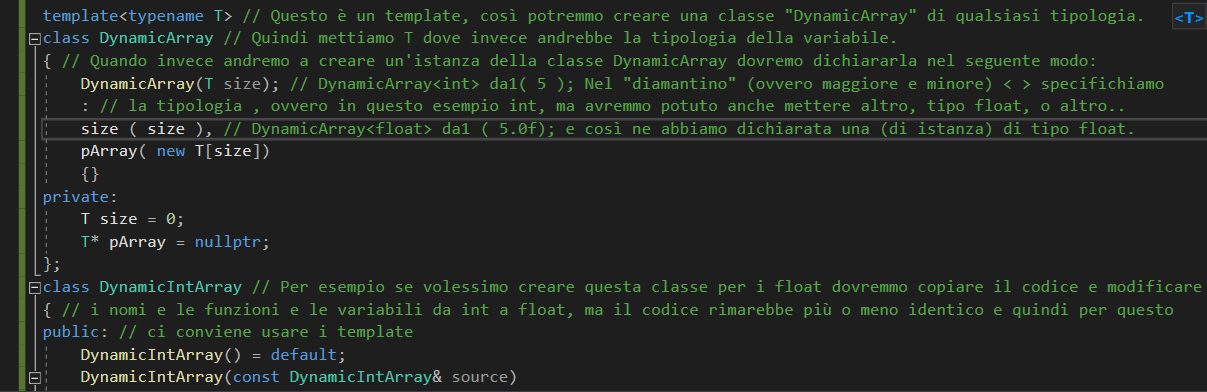
\includegraphics[width=1.2\textwidth, height=1.2\textheight, keepaspectratio]{./imgs/template.png}
	\caption{Template}
	\label{fig:template}
\end{figure}

%TODO: typename

% -------------------------- SECTION: VECTOR -----------------------------------------

%TODO: emplace_back

\section{std::vector<>}

\textsf{\small \textbf{Definizione:} I \textbf{vectors} sono un contenitore rappresentante una array che può cambiare in size (spazio). Sono degli array dinamici.} \\

\textsf{\small I vectors memorizzano i dati in locazioni contigue di memoria e permettono l'accesso diretto a qualsiasi elemento usando l'operatore []. Supportano la riduzione e l'ampiamento dello spazio a runtime (ovvero eseguite mentre il tuo programma è in esecuzione).} \\

\textsf{\small La classe vector fa uso dei template così che possiamo eseguirla con qualsiasi tipo. Per poterla usare avremo bisogno di importare \textbf{\#include <vector>}.} \\

\begin{lstlisting}
	#include <iostream>
	#include <vector>
	
	std::vector<int> v{ 1, 3, 7, 8};
	std::vector<int> v2 = v; // Oppure potevamo scrivere std::vector<int> v2(v);
	
	v2.push_back(9); // Aggiungiamo un elemento.
	
	std::cout << "v size: " << v.size() << std::endl; //Output: v size: 4
	std::cout << "v2 size: " << v2.size() << std::endl; //Output: v2 size: 5
\end{lstlisting}

\textsf{\small Inoltre, la classe vector mette a disposizione tante altre funzioni per la loro manipolazione.} \\

\textsf{\small P.S.: Da non confondere con i vettori in matematica|fisica.} \break

% -------------------------- SECTION: ITERATORI --------------------------------------

\newpage

\section{Iteratori}

\textsf{\small \textbf{Definizione: } Gli \textbf{iteratori} sono degli oggetti (come puntatori) che puntano ad un elemento all'interno di un contenitore. Usiamo gli \textbf{iteratori} per muoverci nel contenitore } \break

\textsf{\small Ci sono diversi tipi di iteratori: } \\

\begin{itemize}
	\item \textsf{\small \textbf{Input Iterators} : Sono i più deboli fra tutti per via delle loro limitate funzionalità. Può essere usato solo in algoritmi single-pass ovvero quelli che processano il contenitore in modo sequenziale.}
	\item \textsf{\small \textbf{Output Iterators} : Anch'essi sono molto limitati. Possono essere usati negli algoritmi single-pass, ma non per accedere agli elementi, ma per essere assegnati agli elementi.}
	\item \textsf{\small \textbf{Forward Iterator} : Sono più in alto nella gerarchia rispetto agli input ed output e possiedono tutte le funzionalità di questi ultimi due, ma possono anche muoversi in avanti ed anch'essi di una posizione alla volta.}
	\item \textsf{\small \textbf{Bidirectional Iterators} : Possiedono tutte le funzionalità degli forward iterators, ma possono muoversi in entrambe le direzioni.}
	\item \textsf{\small \textbf{Random-Access Iterators} : Sono gli iteratori più potenti. Non sono limitati dal solo poter muoversi in modo sequenziale, ma possono accedere in maniera casuale a qualsiasi elemento dentro ad un contenitore. Sono quelli che hanno le stesse funzionalità dei puntatori.}
\end{itemize}

\pagebreak

\begin{figure}[H]
	\centering
	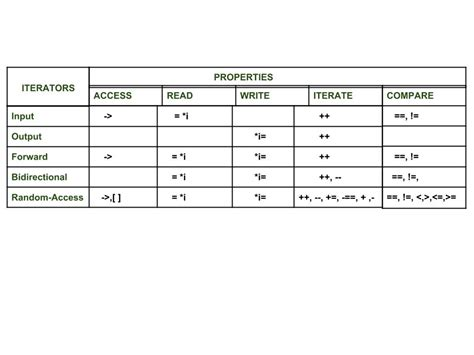
\includegraphics[width=1.2\textwidth, height=1.2\textheight, keepaspectratio]{./imgs/iterators.jpg}
	%\caption{Iteratori}
	\label{fig:iterators}
\end{figure}

\vspace{-3.69cm}

\textsf{\small È sempre meglio usare gli \textbf{iteratori} per iterare tra i contenuti di un contenitore così da evitare di usare l'operatore \textbf{[]} per accedere agli elementi. Inoltre per ottenere la fine di un contenitore con gli \textbf{iteratori} possiamo semplicemente usare la funzione \textbf{end()} al posto di utilizzare lo spazio occupato. } \break

\textsf{\small Possono essere utili per la riusabilità del codice, visto che anche se cambiamo vettore, il codice riguardante gli \textbf{iteratori} non dovrebbe cambiare.} \\

\textsf{\small Gli \textbf{iteratori} ci permettono una manipolazione dinamica dei contenitori, permettendoci di aggiungere e rimuovere elementi in modo dinamico a nostro piacimento.} \break

\textsf{\small Per poter usare gli iteratori è necessario includere \textbf{\#include <iterator>}.} \\

\begin{itemize}
	\item \textsf{\small \textbf{begin()} : Restituisce la posizione iniziale del contenitore.}
	\item \textsf{\small \textbf{end()} : Restituisce la posizione finale del contenitore.}
	%\item \textsf{\small \textbf{} :}
\end{itemize}

\begin{lstlisting}
	#include <iostream>
	#include <iterator>
	
	std::vector<int> v = { 9, 6, 3};
	
	// Dichiaro un iteratore.
	std::vector<int>::iterator it;
	for(it = v.begin(); it < v.end(); it++)
	{
		std::cout << "Elemento: " << *it << std::endl;
	}

	// Output: stampa uno ad uno gli elementi del vettore.
\end{lstlisting}

\begin{itemize}
	\item \textsf{\small \textbf{advance()} : Incrementa la posizione dell'iteratore fino all'argomento passato come parametro.}
	\item \textsf{\small \textbf{next()} : Restituisce un nuovo iteratore dopo aver avanzato di tot posizioni menzionate nell'argomento.}
	\item \textsf{\small \textbf{prev()} : Restituisce un nuovo iteratore dopo essere retrocesso di tot posizioni menzionate nell'argomento.}
	\item \textsf{\small \textbf{inserter()} : Per inserire elementi ad qualsiasi posizione nel contenitore. Prende due argomenti: il contenitore e l'iteratore alla posizione in cui l'elemento deve essere inserito.}
\end{itemize}

\begin{lstlisting}
	#include <iostream>
	#include <iterator>
	
	std::vector<int> v = { 9, 6, 3};
	std::vector<int> v2(2, 5, 8);
	
	std::vector<int>::iterator it = v.begin();
	
	std::advance(it, 2);
	
	std::cout << "Elemento dell'iteratore dopo advance: " << *it << std::endl; // Output: Elemento dell'iteratore dopo advance: 3
	
	std::prev(it, 2);
	std::cout << "Elemento dell'iteratore dopo prec: " << *it << std::endl; // Output: Elemento dell'iteratore dopo prec: 9
	
	std::next(it, 1);
	std::cout << "Elemento dell'iteratore dopo next: " << *it << std::endl; // Output: Elemento dell'iteratore dopo next: 6
	
	// Copio gli elementi di 1 vettore nell'altro usando inserter
	// Inserisco gli elementi di v2 in v alla posizione a cui puntava l'iteratore it.
	std::copy(v2.begin(), v2.end(), std::inserter(v, it));
	
	for(int &x : v)
	{
		std::cout << "Elemento: " << x << std::endl;
	}

	// Output: Gli elementi del vettore con gli elementi aggiunti.
\end{lstlisting}

%TODO: Iterable Interface?

% -------------------------- SECTION: VIRTUAL ----------------------------------------

\newpage

\section{Virtual}

\subsection{Virtual functions}

\textsf{\small \textbf{Definizione:} Una funzione \textbf{virtuale} è una funzione dichiarata in una classe base che può essere ri-definita (\emph{overridden}) da una classe derivata. Le funzioni \textbf{virtuali} ci assicurano che la corretta versione della funzione venga eseguita.} \\

\textsf{\small Alcune regole per le \textbf{funzioni virtuali}: }

\begin{itemize}
	\item \textsf{\small Non possono essere statiche.}
	\item \textsf{\small Può essere una \textbf{friend function} di un'altra classe.}
	\item \textsf{\small Bisognerebbe accedergli attraverso un puntatore o referenza di un tipo alla classe base per ottenere \emph{runtime polymorphism}.}
	\item \textsf{\small Il prototipo della funzione dovrebbe essere lo stesso sia nella classe base sia nella classe derivata.}
	\item \textsf{\small Sono sempre definiti nella classe base e ridefiniti nella classe derivata. Non è obbligatorio che la classe derivata ri-definisca la funzione, può anche soltanto utilizzare quella della classe base.}
	\item \textsf{\small Una classe può avere un \textbf{virtual destructor}, ma non un \textbf{virtual constructor}.}
\end{itemize}

\begin{lstlisting}
	#include <iostream>
	
	class Base {
		public:
			virtual void print()
			{
				std::cout << "print in base class" << std::endl;
			}
		
			void show()
			{
				std::cout << "show in base class" << std::endl;
			}
	};

	class Derived : public Base {
		public:
			void print() override // override non servirebbe, ma aiuta per la manutenzione del codice ed indica che la funzione è stata "overridata".
			{
				std::cout << "print in derived class" << std::endl;
			}
		
			void show()
			{
				std::cout << "show in derived class" << std::endl;
			}
	};

	int main()
	{
		Base* bPtr;
		Derived d;
		bPtr = &d;
		
		// Chiamo la funzione virtuale.
		bPtr->print(); // Output: print in derived class
		
		// Chiamo la funzione non virtuale.
		bPtr->show(); // Output: show in base class
		
		return 0;
	}
\end{lstlisting}

\subsection{Virtual Destructors}

\textsf{\small \textbf{Definizione:} Per rimuovere una classe derivata, la classe base dovrebbe essere definita con un \textbf{distruttore virtuale}. Cancellare una classe derivata usando un puntatore alla classe base senza un distruttore virtuale risulta in un comportamento indefinito (\emph{undefined behaviour}).} \\

\begin{lstlisting}
	#include <iostream>
	
	class A {
		public:
			A()
			{
				std::cout << "Constructor in base class" << std::endl;
			}	
		
			virtual ~A()
			{
				std::cout << "Destructor in base class" << std::endl;
			}
	};

	class B : public A {
		public:
			B()
			{
				std::cout << "Constructor in derived class" << std::endl;
			}
		
			~B()
			{
				std::cout << "Destructor in derived class" << std::endl;
			}
	};

	int main()
	{
		B* bPtr = new B();
		A* aPtr = bPtr;
		
		delete aPtr;
		
		// Output: 
		// Constructor in base class
		// Constructor in derived class
		// Destructor in derived class
		// Destructor in base class
		return 0;
	}
\end{lstlisting}

\textsf{\small In linea di massima, se si ha una funzione virtuale, allora è da mettere anche il distruttore virtuale.} \break

\subsection{Virtual Inheritance}

\textsf{\small \textbf{Definizione:} La \textbf{Ereditarietà virtuale} è usata per risolvere il problema del \textbf{DDD} (\emph{Dreadful Diamond on Derivation}), ovvero quando una classe deriva molteplici classi che derivano dalla stessa classe.} \\

\begin{figure}[H]
	\centering
	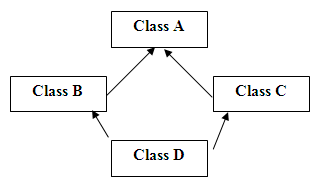
\includegraphics[width=1\textwidth, height=1\textheight, keepaspectratio]{./imgs/diamond_problem2.png}
	\caption{Problema del diamante}
	\label{fig:diamond_problem}
\end{figure}

\textsf{\small Come possiamo notare i dati e le funzioni della \textbf{classe A} è ereditata due volte dalla \textbf{classe D}, una volta per via della \textbf{classe B} e una volta per via della \textbf{classe C}.} \\

\textsf{\small Quando qualsiasi dato o funzione della \textbf{classe A} viene acceduto dalla \textbf{classe D}, nasce dell'ambiguità su quale dato/funzione chiamare. Quella ereditata da \textbf{B} o da \textbf{C}? Questo confonde i compilatori e mostrano errori.}

\textsf{\small Per risolvere questa ambiguità quando la \textbf{classe A} è ereditata sia dalla \textbf{classe B} sia dalla \textbf{classe C}, è dichiarata come \textbf{classe base virtuale} (Fare riferimento all'immagine: \textbf{\ref{fig:diamond_problem}} a \textbf{pag.\pageref{fig:diamond_problem}}).}

\begin{lstlisting}
	#include <iostream>
	
	class A {
		public:
			void show()
			{
				std::cout << "Show from A" << std::endl;
			}
	};

	class B : public virtual A {
	};

	class C : public virtual A {
	};

	class D : public B, public C {
	};

	int main()
	{
		D d;
		d.show(); // Output: Show from A
	}
\end{lstlisting}

\textsf{\small La keyword \textbf{virtual} può essere posta sia prima che dopo \textbf{public}.} \\

%TODO: Aggiungere immagini: "virtual_functions_recap_terminology_and_concepts".
%TODO: Aggiungere immagini: "virtual_functions_implementation".

% -------------------------- SECTION: POLYMORPHISM -----------------------------------

\section{Polimorfismo}

\textsf{\small \textbf{Definizione:} La parola \textbf{polimorfismo} significa \emph{avere molte forme}, questo occorre quando c'è una gerarchia di classi e queste sono correlate attraverso l'ereditarietà.} \\

\textsf{\small Ci sono due tipi principali di polimorfismo: }

\begin{itemize}
	\item \textsf{\small \textbf{Compile time Polymorphism} : si ottiene dall'\emph{overloading} di funzioni o di operatori.}
	\item \textsf{\small \textbf{Runtime Polymorphism} : si ottiene dall' \emph{overriding} delle funzioni (con la keyword \textbf{virtual}).}
\end{itemize}

\begin{figure}[H]
	\centering
	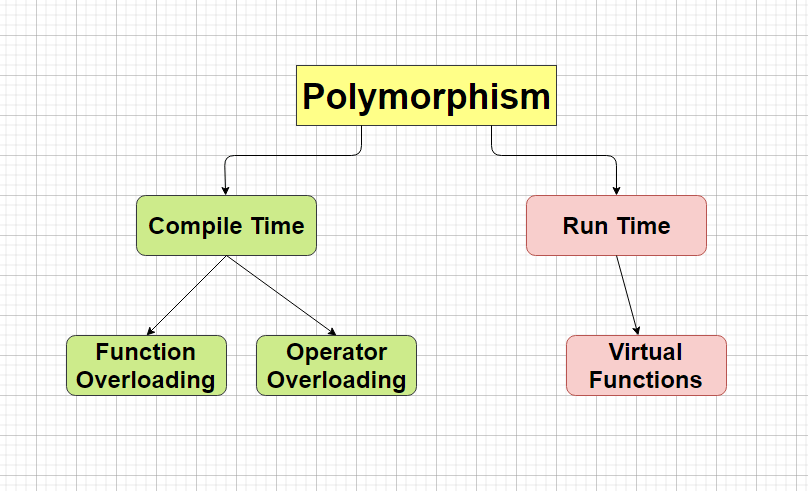
\includegraphics[width=1\textwidth, height=1\textheight, keepaspectratio]{./imgs/polymorphism.png}
	\caption{Polimorfismo}
	\label{fig:polymorphism}
\end{figure}

% -------------------------- SECTION: OVERLOADING ------------------------------------

\section{Overloading}

\textsf{\small \textbf{Definizione:} L'\textbf{overloading} permette di ridefinire una funzione o un operatore con lo stesso nome e nello stesso scope, ma con una differente implementazione.} \\

\subsection{Function Overloading}

\textsf{\small Si può definire una funzione con lo stesso nome di un'altra purchè abbia argomenti diversi.} \\

\begin{lstlisting}
	void func(int x)
	{
		std::cout << "Valore di x: " << x << std::endl;
	}

	void func(double x)
	{
		std::cout << "Valore di x: " << x << std::endl;
	}

	void func(float x)
	{
		std::cout << "Valore di x: " << x << std::endl;
	}
\end{lstlisting}

\subsection{Operator Overloading}

\textsf{\small Possiamo ridefinire degli operatori per eseguire delle operazioni nel modo che vogliamo noi.} \\

\textsf{\small Utilizziamo la keyword \textbf{operator} ed il simbolo dell'operatore per \emph{overloaddarlo}.} \\

\begin{lstlisting}
	class Vec {
		public:
			Vec(){}
		
			Vec(int x, int y)
			{
				this->x = x;
				this->y = y;
			}
		
			Vector operator+(const Vec& v)
			{
				Vec vec;
				vec.x = this->x + v.x;
				vec.y = this->y + v.y;
				return vec;
			}
		
			int getX()
			{
				return this->x;
			}
		
			int getY()
			{
				return this->y;
			}
		
		private:
			int x;
			int y;
	};

	int main()
	{
		Vec v1(3, 2);
		Vec v2(1, 0);
		
		Vec v3 = v1 + v2;
		
		std::cout << "v3.x: " << v3.getX() << "; v3.getY(): " << v3.y << std::endl;
		// Output: v3.x: 4; v3.y: 2
		// perché facciamo la x di v1 che è 3 + la x di v2 che è 1 quindi 4 e 
		// la y di v1, ovvero 2 + la y di v2, ovvero 0 quindi 2
		// quindi v3 ha membri (4,2).
		return 0;
	}
\end{lstlisting}

\textsf{\small Non tutti gli operatori si possono \emph{overloaddare}.} \\

\textsf{\small Gli operatori che non si possono \emph{overloaddare} sono: \textbf{.} (punto), \textbf{::}, \textbf{?:}(operatore ternario), \textbf{sizeof}.} \\

\subsection{Overloading vs Overriding}

\textsf{\small L'\textbf{overloading} è la creazione di molteplici definizioni di una funzione cambiando la \textbf{signature}: il numero di parametri, la tipologia dei parametri. Il tipo di ritorno non gioca alcun ruolo.} \\

\textsf{\small Può essere fatta sia nelle classi basi che in quelle derivate.} \break

\textsf{\small L'\textbf{overriding} è la ridefinizione di una funzione di una classe base in una classe derivata con la stessa \textbf{signature}, stesso tipo di ritorno e parametri.} \\

\textsf{\small Può essere fatta solo nelle classi derivate.} \break

\textsf{\small Differenza tra \textbf{function overloading} e \textbf{function overriding}: } \break

\begin{tabular}{|c|c|} %TODO: questo è da riguardare, perché la fonte forse ha fatto degli errori.
	\hline
	\textbf{Overloading} & \textbf{Overriding} \\
	\hline
	\textsf{\small Nessuna keyword è usata.} & \textsf{\small Keyword \textbf{override}.} \\
	\hline
	\textsf{\small Il prototipo cambia } & \textsf{\small Il prototipo non cambia.} \\
	\textsf{\small in base ai parametri.} & \textsf{\small } \\
	\hline
	\textsf{\small Occorre durante compile time.} & \textsf{\small Occorre durante runtime.} \\
	\hline
	\textsf{\small I costruttori possono } & \textsf{\small } \\
	\textsf{\small essere "overloaddati".} & \textsf{\small } \\
	\hline
	\textsf{\small I distruttori non } & \textsf{\small I distruttori } \\
	\textsf{\small possono essere "overloaddati".} & \textsf{\small possono essere "overridati".} \\
	\hline
	\textsf{\small } & \textsf{\small Le funzioni virtuali } \\
	\textsf{\small } & \textsf{\small non possono essere "overridate".} \\
	\hline
	\textsf{\small Può essere usato per ottenere } & \textsf{\small Overriding è anche conosciuto come } \\
	\textsf{\small \emph{early binding}.} & \textsf{\small \emph{late binding}.} \\
	\hline
	\textsf{\small La funzione chiamata viene } & \textsf{\small La funzione overriden} \\
	\textsf{\small determinata dal numero} & \textsf{\small è preceduta} \\
	\textsf{\small di parametri.} & \textsf{\small dalla keyword virtual nella classe base.} \\
	\hline
	\textsf{\small Le funzioni verrebbero} & \textsf{\small } \\
	\textsf{\small ridefinite} & \textsf{\small } \\
	\textsf{\small con lo stesso nome, ma} & \textsf{\small } \\
	\textsf{\small differente numero o tipo} & \textsf{\small } \\
	\textsf{\small di parametri.} & \textsf{\small } \\
	\hline
	\textsf{\small } & \textsf{\small L'indirizzo dell'oggetto} \\
	\textsf{\small } & \textsf{\small della classe è assegnato al} \\
	\textsf{\small } & \textsf{\small puntatore la cui funzione} \\
	\textsf{\small } & \textsf{\small è chiamata dal puntatore.} \\
	\hline
	\textsf{\small } & \textsf{\small Quando la funzione è definita viene preceduta} \\
	\textsf{\small } & \textsf{\small dalla keyword virtual nel main.} \\
	%\textsf{\small } & \textsf{\small La stessa funzione è ridefinita } \\
	%\textsf{\small } & \textsf{\small nella classe derivata usando} \\
	%\textsf{\small } & \textsf{\small la keyword \textbf{out}.} \\
	%\textsf{\small } & \textsf{\small } \\
	\hline
\end{tabular}

% -------------------------- SECTION: TIPI DI CAST -----------------------------------

\newpage

\section{Tipi di Casts}

\textsf{\small \textbf{Definizione:} Il \textbf{casting} è un'operazione che permette la conversione di un valore in un altro. In C++ ci sono diversi tipi di casting: } \\

\subsection{static\_cast<>}

\begin{itemize}
	\item \textsf{\small \textbf{static\_cast<> :} Quello che fa è un cast implicito tra tipi (come int a float, o puntatore a void*) e può anche chiamare funzioni esplicite per la conversione. }
\end{itemize}

\begin{lstlisting}
	float f = 3.69;
	int x = static_cast<int>(f);
	std::cout << "x: " << x << std::endl; // Output: x: 3 
\end{lstlisting}

\subsection{const\_cast<>}

\begin{itemize}
	\item \textsf{\small \textbf{const\_cast<> :} Serve per aggiungere o rimuovere il \textbf{const} ad una variabile. Se la variabile che stiamo cercando di modificare era già const allora questo produce un valore indefinito. Se lo si usa per qualcosa che non era dichiarato come const allora è safe (sicuro farlo, non ci saranno problemi).  }
\end{itemize}

\begin{lstlisting}
	#include <iostream>
	
	void print( char* str)
	{
		std::cout << str << '\n';
	}

	int main()
	{
		const char* c = "testo";
		// Ci serve per poter passare un puntatore a char const ad una funzione che prende un puntatore a char senza const.
		print(const_cast<char*>(c)); // Output: testo
		return 0;
	}
\end{lstlisting}

\subsection{dynamic\_cast<>}

\begin{itemize}
	\item \textsf{\small \textbf{dynamic\_cast<> :} Serve esclusivamente per i casts riguardanti il polimorfismo. Puoi castare un puntatore o una reference a qualsiasi altro tipo di classe. Non solo si può fare un casting verso il basso, ma anche in alto e a lato. Il dynamic\_cast cercherà di ritorna l'oggetto desiderato se possibile, altrimenti ritornerà \textbf{nullptr} in caso di un puntatore e \textbf{std::bad\_cast} nel caso di una reference.}
	\item \textsf{\small Ha delle limitazioni. Non funzionerà nel caso in cui diversi oggetti ereditano tutti dallo stessa classe. (il famoso problema del \emph{dreaded diamond}.) e non stai usando l'ereditarietà \textbf{virtual}.}
	\item \textsf{\small Inoltre può soltanto funzionare con l'ereditarietà pubblica, fallirà con l'ereditarietà \textbf{protected} o \textbf{private}. Comunque questi tipi di ereditarietà sono rare.}
\end{itemize}

\begin{lstlisting}
	// C++ programma per dimostrare che se non c'è
	// alcuna funzione virtuale nella Base classe.
	#include <iostream>
	
	// Base class declaration
	class Base {
		void print()
		{
			std::cout << "Base" << std::endl;
		}
	};
	
	// Derived Class 1 declaration
	class Derived1 : public Base {
		void print()
		{
			std::cout << "Derived1" << std::endl;
		}
	};
	
	// Derived class 2 declaration
	class Derived2 : public Base {
		void print()
		{
			std::cout << "Derived2" << std::endl;
		}
	};
	
	// Driver Code
	int main()
	{
		Derived1 d1;
		
		// Base class pointer hold Derived1
		// class object
		Base* bp = dynamic_cast<Base*>(&d1);
		
		// Dynamic casting
		Derived2* dp2 = dynamic_cast<Derived2*>(bp);
		if (dp2 == nullptr)
			std::cout << "null" << std::endl;
			
		// Output: null, in realtà errore.
		return 0;
	}
\end{lstlisting}

\subsection{reinterpret\_cast<>}

\begin{itemize}
	\item \textsf{\small \textbf{reinterpret\_cast<> :} È quello più pericoloso di tutti e quindi bisogna utilizzarlo con moderazione. Trasforma un tipo direttamente in un altro come cast da un puntatore ad un altro o memorizzare un puntatore in un int, ecc..}
	\item \textsf{\small L'unica cosa garantita con questo tipo di cast è che se torni indietro al tipo originale riotterrai lo stesso valore (non succederà se il tipo era più piccolo del tipo originale.)}
\end{itemize}

\begin{lstlisting}
	class A {
		public:
			int x;
	};

	class B {
		public:
			int x;
	};

	A *a = new A;
	B *b = reinterpret_cast<*B>(a);
	
	a->x = 5;
	std::cout << "b: " << b->x << std::endl; // Output: b: 5
	std::cout << "a: " << a->x << std::endl; // Output: a: 5
\end{lstlisting}

\subsection{C-style \& function-style cast o Regular Cast}

\begin{itemize}
	\item \textsf{\small Questo tipo di cast chiamato \textbf{Regular Cast} o \textbf{C-style cast} (derivando dal C ovviamente) è molto più potente degli altri tipi di cast, ma allo stesso tempo molto meno sicuro.}
	\item \textsf{\small Ignorano i controlli d'accesso quando si esegue uno static\_cast.}
	\item \textsf{\small Permette di fare un cast sicuro ad una classe privata, mentre il suo "equivalente" static\_cast darebbe un errore a tempo di compilazione (compile-time).}
\end{itemize}

\begin{lstlisting}
	double d = 9.87;
	int x;
	
	x = (int)d;
	std::cout << "x: " << x std::endl; // Output: x: 9
\end{lstlisting}

\subsection{Ricapitolando}

\begin{tabular}{|c|c|}
	\hline
	\textbf{Cast} & \textbf{Definizione} \\
	\hline
	\textbf{dynamic\_cast} & \textsf{\small per convertire puntatori/references in una gerarchia di ereditarietà.} \\
	\hline
	\textbf{static\_cast} & \textsf{\small per le conversioni di tipi ordinari.} \\
	\hline
	\textbf{reinterpret\_cast} & \textsf{\small per reinterpretare bit patterns di basso livello. Usare con cauzione.} \\
	\hline
	\textbf{const\_cast} & \textsf{\small per aggiungere/rimuovere \textbf{const} al cast.} \\
	\hline
\end{tabular}

\begin{figure}[ht]
	\centering
	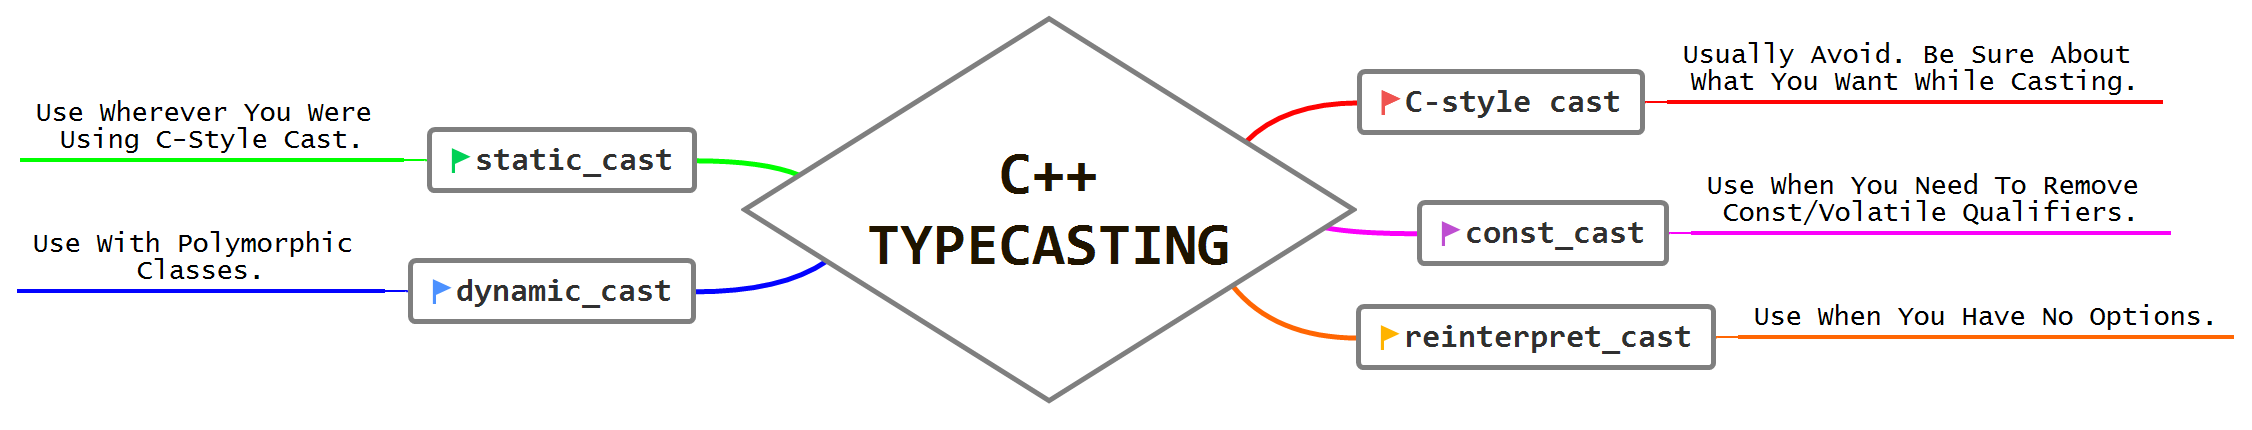
\includegraphics[width=1.2\textwidth, height=1.2\textheight, keepaspectratio]{./imgs/typecasting.png}
	\caption{Typecasting}
	\label{fig:typecasting}
\end{figure}

%TODO: Aggiungere immagine "cast_types_recap_static_dynamic_reinterpret_const_c-style".

%TODO: typeid

% -------------------------- SECTION: LAMBDAS ----------------------------------------

%TODO: potrei mettere le lambbdas subito dopo gli iteratori.

\section{Lambdas}

\textsf{\small \textbf{Definizione:} Dal C++11 sono presenti le \textbf{lambdas} che permettono di creare \textbf{funzioni anonime}.} \\

\textsf{\small Servono per creare delle funzioni, dei piccoli frammenti di codice che non hanno bisogno di un nome e non verranno riutilizzati. } \\ % funzioni inline

\textsf{\small Sono una parte centrale della \textbf{programmazione funzionale}.} \\

\textsf{\small Questa è la struttura di una tipica espressione \textbf{lambda} :} \\

\begin{lstlisting}
	[ clausola di cattura ] ( lista di parametri che è opzionale) -> tipoDiRitorno
	{
		// Definizione della lambda.
	}
\end{lstlisting}

\textsf{\small Se nella clausola della cattura è presente un \textbf{=} (uguale), vuol dire che la lambda può accedere a qualsiasi variabile, se c'è un \textbf{\&} vuol dire che stiamo accedendo alle variabili per reference, se la clausola [] è vuota allora può accedere soltanto alle variabili locali, altrimenti lì saranno presenti i nomi delle variabili che si vogliono utilizzare ("catturate" o per valore o per reference).} \\ %TODO: forse si potrebbe rimuovere questa parte e lasciare solo la tabella.

\begin{tabular}{|c|c|}
	\hline
	\textbf{Cattura} & \textbf{Definizione} \\
	\hline
	\textsf{\small []} & \textsf{\small accedere solo alla variabili locali} \\
	\hline
	\textsf{\small [=]} & \textsf{\small accedere a tutte le variabili per valore.} \\
	\hline
	\textsf{\small [\&]} & \textsf{\small accedere a tutte le variabili per reference.} \\
	\hline
	\textsf{\small [nomeVariabile1, \&nomeVariabile2]} & \textsf{\small "cattura" nomeVariabile per valore } \\
	\textsf{\small } & \textsf{\small e nomeVariabile2 per referenza.} \\
	\hline
\end{tabular} \\

\begin{lstlisting}
	#include <iostream>
	#include <vector>
	
	std::vector<int> v1 = { 5, 8, 9, 1, 7};
	std::vector<int> v2 = {12, 36, 27, 92};
	
	// Lambda.
	auto pushinto = [&](int m)
	{
		v1.push_back(m);
		v2.push_back(m);
	}; // Da notare il ; alla fine.

	// Pusha in entrambi v1 e v2 il numero 24
	pushinto(24);
	
	// Lambda, accediamo a v1 per valore (quindi ne facciamo una copia).
	[v1]()
	{
		for(auto p = v1.begin(); p != v1.end(); p++)
		{
			std::cout << *p << std::endl;
		}
	};

	int n = 7;
	// trova il primo numero maggiore di n.
	// [n] significa che stiamo accedendo e possiamo soltanto accedere ad n (per valore, ovvero una copia di essa).
	std::vector<int>:: iterator p = std::find_if(v1.begin(), v1.end(), [n](int i)
	{
		return i > n;
	});

	std::cout << "Il primo numero maggiore di n e\': " << *p << std::endl; // Output: Il primo numero maggiore di n e\': 8

	// Qui [=] vuol dire che possiamo accedere a tutte le variabili.
	int countN = std::count_if(v1.begin(), v1.end(), [=](int a) 
	{
		return a >= n;
	});

	std::cout << "Il numero di elementi piu' grandi o uguali ad n sono: " << countN << std::endl; // Output: Il numero di elementi più grandi o uguali ad n sono: 4 (perchè abbiamo inserito anche il 24 nell'operazione precedente).
\end{lstlisting}

%TODO: capture.
%TODO: poi trattare anche dei functors.

% -------------------------- SECTION: MEMORIA DINAMICA -------------------------------

\newpage

\section{Memoria dinamica}

\textsf{\small \textbf{Definizione: } Riguarda l'allocazione di memoria manualmente da parte del programmatore. La memoria allocata dinamicamente è allocata nell' \textbf{Heap} mentre le variabili locali e la memoria non statica viene allocata nello \textbf{Stack}.}

\begin{itemize}
	\item \textsf{\small \textbf{Heap} : memoria dinamica.}
	\item \textsf{\small \textbf{Stack} : variabili locali e non-statiche.}
\end{itemize}

\subsection{Memoria Dinamica in C}

\textsf{\small In C per l'allocazione dinamica della memoria usufruivamo di 4 diverse funzioni: \textbf{malloc()} (per allocare), \textbf{calloc()}, \textbf{realloc()} (per riallocare), \textbf{free()} (per liberare la memoria).} \\

\textsf{\small Tutte questi funzioni del C, esistono anche nel C++, ma questo ha un suo modo per l'allocazione dinamica della memoria.} \break

\subsection{new e delete}

\subsubsection{new}

\textsf{\small \textbf{Definizione: } L'operatore \textbf{new} denota una richiesta di allocazione di memoria nello spazio libero. Se sufficiente memoria è disponibile, l'operatore inizializza la memoria e restituisce l'indirizzo della nuova memoria allocata ed inizializzata al puntatore.} \\

\begin{lstlisting}
	// Esempio 1
	int *ptr = nullptr;
	ptr = new int;
	
	// Esempio 2
	double *dPtr = new double;
	
	// Esempio 3
	int *p = new int(22);
	
	// Esempio 4
	int *pArray = new int[12];
\end{lstlisting}

\subsubsection{array normali vs array con la new}

\textsf{\small L'unica differenza è che gli array normali vengono deallocati dal compilatore, mentre quelli creati con la new devono essere deallocati dal programmatore.} \break

\subsubsection{delete}

\textsf{\small \textbf{Definizione: } Utilizziamo la keyword \textbf{delete} per deallocare la memoria precedentemente allocata.} \\

\begin{lstlisting}
	// Esempio 1
	int *ptr = new int;
	
	delele ptr;
	
	// Esempio 2
	int *p = new int[6];
	
	delete[] p;
\end{lstlisting}

\subsection{Evitare di usare new}

\textsf{\small \textbf{Definizione: } Ci sono vari motivi per cui evitare o minimizzare gli utilizzi della keyword \textbf{new}: } \\

\begin{itemize}
	\item \textsf{\small Il C++ non ha un garbage collector, quindi per ogni \textbf{new} ci deve essere una corrispondente \textbf{delete}.}
	\item \textsf{\small Se viene lanciata un'eccezione poi la memoria non viene mai liberata.}
	\item \textsf{\small Dovrebbe essere tutto nel distruttore, concetto del \emph{RAII}.} %TODO: add ref quando ne parlerò.
	\item \textsf{\small Se restituisci per esempio una stringa a qualcuno, ora sono loro a doverla cancellare (con la \textbf{delete}). E se a loro volta la passassero come argomento? Quando dovrebbe essere liberata? (con \textbf{delete}).}
	\item \textsf{\small Può essere un problema nel multi-threading.}
	\item \textsf{\small Potrebbe portare a dei \emph{memory leaks}.}
\end{itemize}

% -------------------------- SECTION: RAII -------------------------------------------

\section{RAII | Resource Acquisition is initialization}

\textsf{\small \textbf{Definizione: } \textbf{RAII} (\emph{Resource Acquisition is Initialization}) è un idioma comune della programmazione e della gestione delle risorse. Ogni allocazione della risorsa è fatta alla creazione dell'oggetto da parte del \textbf{costruttore} mentre la deallocazione (rilascio della memoria) viene fatto dal \textbf{distruttore}. Quindi se non ci sono leaks all'oggetto, non ci sono leaks nemmeno alla risorse. } \\

\begin{figure}[ht]
	\centering
	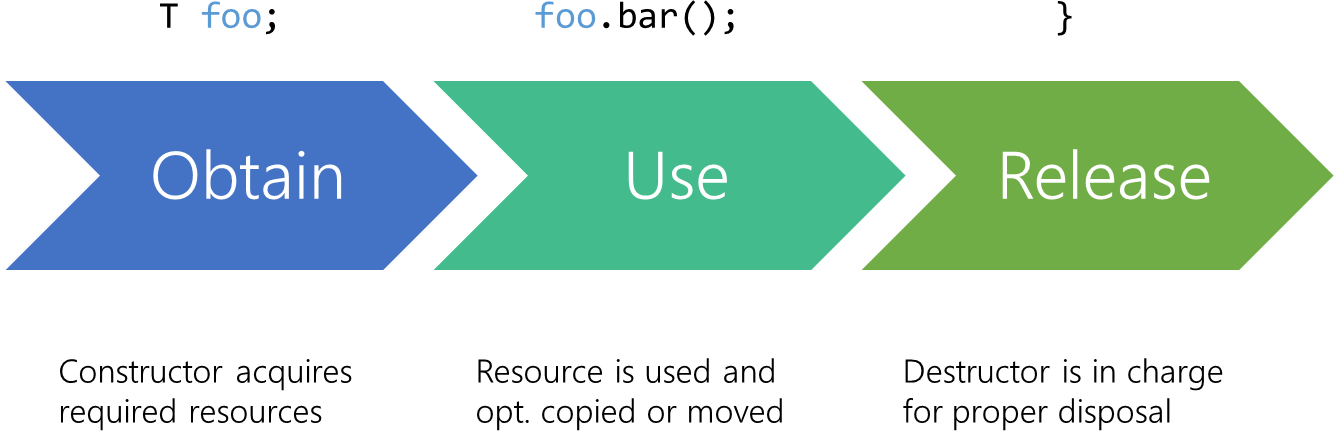
\includegraphics[width=1\textwidth, height=1\textheight, keepaspectratio]{./imgs/RAII.png}
	\caption{RAII}
	\label{fig:RAII}
\end{figure}

%TOOD: magari approfondire l'argomento.

% -------------------------- SECTION: TIPI DI COSTRUTTORI | RULE OF 3 ----------------

\section{Constructor types | Rules of}

\subsection{Rule of Zero}

\textsf{\small \textbf{Definizione: } La \textbf{regola dello zero} (è una regola generale/un'indicazione) afferma che se non hai bisogno di nessuno di questi, allora non ne devi implementare nessuno: } \\

\begin{itemize}
	\item \textsf{\small \textbf{Distruttore} : libera tutte le risorse precedentemente allocate.}
	\item \textsf{\small \textbf{Copy Constructor} : Fa una copia di un oggetto.}
	\item \textsf{\small \textbf{Copy assign} : overload dell'operatore di assegnamento.}
\end{itemize}

\subsection{Copy Constructor}

\textsf{\small \textbf{Definizione: } Il \textbf{Copy Constructor} è un tipo di costruttore che inizializza un oggetto usando un altro oggetto della stessa classe.} \\

\textsf{\small Un costruttore di copia ha la seguente struttura: } \\

\begin{lstlisting}
	// È un costruttore quindi si chiama con il nome della classe.
	NomeDellaClasse(const NomeDellaClasse &vecchioOggetto);
\end{lstlisting}

\textsf{\small Un copy constructor potrebbe essere chiamato per:}

\begin{enumerate}
	\item \textsf{\small Quando un oggetto della classe è ritornato per valore.}
	\item \textsf{\small Quando un oggetto della classe è passato come argomento ad una funzione per valore.}
	\item \textsf{\small Quando un oggetto è costruito sulla base di un altro oggetto.}
	\item \textsf{\small Quando il compilatore genera un oggetto temporaneo.}
	%\item \textsf{\small }
\end{enumerate}

\begin{lstlisting}
	class Point {
		public:
			// Costruttore normale
			Point(int x, int y)
			{
				this->x = x;
				this->y = y;
			}
			
			// Copy Constructor
			// Assiegnamo i valori di x ed y in base ai valori di un'istanza p della classe Point.
			Point(const Point &p)
			{
				this->x = p.x;
				this->y = p.y;
			}
		
			int getX() { return this->x };
			int getY() { return this->y };
		
		private:
			int x;
			int y;
	};

	int main()
	{
		Point p1(3, 5); // Il costruttore normale viene chiamato qui.
		Point p2 = p1; // Il Copy Constructor viene chiamato qui.
		
		std::cout << "p1.x: " << p1.getX() << ", p1.y: " << p1.getY() << "\n"; // Output: p1.x: 3, p1.y: 5
		std::cout << "p2.x: " << p2.getX() << ", p2.y: " << p2.getY() << "\n"; // Output: p2.x: 3, p2.y: 5
		
		return 0;
	}
\end{lstlisting}

\subsection{Copy Assign}

\textsf{\small \textbf{Definizione: } Il \textbf{copy assignment operator} è ciò che ti permette di assegnare, di copiare un'istanza e di portare i suoi dati in un' altra istanza.} \\

\textsf{\small È usato per rimpiazzare i dati di un oggetto precedentemente inizializzato con i dati di qualche altro oggetto.} \\

\textsf{\small Se non si dichiara un \textbf{assignment operator} allora il compilatore provvederà a fornirtene uno automaticamente.} \\

\textsf{\small In linea di massima, se hai bisogno di un \textbf{copy constructor} allora avrai bisogno anche di un \textbf{copy assignment operator}.} \\

%TODO: da riguardarsi il copy assignment operator nel codice.
\begin{lstlisting}
	class Point {
		public:
			// Normal Constructor
			Point(int x, int y)
			{
				this->x = x;
				this->y = y;
			}
		
			// Copy Constructor
			Point(const Point& p)
			{
				this->x = p.x;
				this->y = p.y;
			}
		
			// Copy Assignment
			Point& operator=(const Point& p)
			{
				this->x = p.x;
				this->y = p.y;
				return *this;
			}
			
			int getX() { return this->x };
			int getY() { return this->y };
			
		private:
			int x;
			int y;
	};
\end{lstlisting}

%TODO: copy constructor = delete, copy assignment = delete.

\subsection{=default | Defaulted Functions}

\textsf{\small \textbf{Definizione: } Le \textbf{defaulted functions} in modo esplicito permette di aggiungere \textbf{=default} alla fine di una funzione per dichiararla una \emph{funzione default esplicita}. Questi sono più efficienti.} \\

\begin{lstlisting}
	class A {
		public:
		A(int a)
		{
			this->a = a;
			this->b = 0;
		}
	
		A(int a, int b) = default
		{
			this->a = a;
			this->b = b;
		};
	
		// Non ci sarebbe bisogno di mettere =default al costruttore A(), perché questo è già il costruttore di default.
		A(); 
		
		int a;
	};

	int main()
	{
		// Eseguito usando il default constructor
		A a(2);
		
		// Eseguito usando il costruttore parametrizzato.
		A b(5, 7);
		return 0;
	}
\end{lstlisting}

\subsection{=delete | Deleted Functions}

\textsf{\small \textbf{Definizione: } Apparte, deallocare la memoria, dal C++11 la \textbf{delete} ha un nuovo significato: \emph{disabilitare l'utilizzo di una funzione membra}. Queste funzioni sono conosciute come \textbf{funzioni deleted esplicitamente}.} \\

\begin{lstlisting}
	class A {
		public:
			A(int a): x(a)
			{
				this->a = a;
			}
		
			// Disabilitare il copy constructor.
			A(const A& ) = delete;
			
			// Disabilitare il copy assignment operator.
			A& operator=(const A& ) = delete;
			
			int x;
	};

	int main()
	{
		A a1(3), a2(6), a3(9);
		
		// Errore, l'utilizzo del copy assignment operator è disabilitato.
		a1 = a2;
		
		// Errore, l'utilizzo del copy constructor è disabilitato.
		a3 = A(a2);
		return 0;
	}
\end{lstlisting}

\textsf{\small \textbf{Ma qual è l'utilità di far ciò?}} \\

\begin{enumerate}
	\item \textsf{\small Previene il compilatore dal generare le \textbf{special member functions} (costruttori, distruttori, copy constructor, ecc..) che non vogliamo.} \\
	\item \textsf{\small Il disabilitare le normali funzioni membro o non-membro previene problemi di promozioni di tipo dal causare una chiamata involontaria alla funzione.} \\
	%\item \textsf{\small } \\
\end{enumerate}

\subsection{Copy Constructor vs Copy Assignment Operator}

\begin{tabular}{|c|c|}
	\hline
	\textbf{Copy Constructor} & \textbf{Copy Assignment Operator} \\
	\hline
	\textsf{\small È chiamato quando una } & \textsf{\small È chiamato quando ad un oggetto } \\
	\textsf{\small nuova istanza viene creata da } & \textsf{\small già inizializzato gli viene } \\
	\textsf{\small un oggetto già esistente, } & \textsf{\small assegnato un nuovo valore } \\
	\textsf{\small come copia di questo.} & \textsf{\small da un oggetto già esistente.} \\
	\hline
	\textsf{\small Crea un nuovo blocco di memoria} & \textsf{\small Non crea un nuovo blocco di memoria.} \\
	\textsf{\small per il nuovo oggetto.} & \textsf{\small } \\
	\hline
	\textsf{\small È un costruttore overloaded.} & \textsf{\small È un operatore bitwise.} \\
	\hline
	\textsf{\small Il compilatore fornisce} & \textsf{\small Una copia bitwise viene creata} \\
	\textsf{\small implicitamente un copy constructor} & \textsf{\small se l'assignment operator} \\
	\textsf{\small se uno non ne esiste già.} & \textsf{\small non viene overloaded.} \\
	%\textsf{\small } & \textsf{\small } \\
	\hline
\end{tabular}

\subsection{Rule of Three}

\textsf{\small \textbf{Definizione: } La \textbf{regola dei tre}, essenzialmente, afferma che se uno (o anche più) tra questi è definito, allora tutti e tre dovrebbero essere definiti: } \\

\begin{itemize}
	\item \textsf{\small \textbf{Distruttore} : libera tutte le risorse precedentemente allocate.}
	\item \textsf{\small \textbf{Copy Constructor} : Fa una copia di un oggetto.}
	\item \textsf{\small \textbf{Copy assignment operator} : overload dell'operatore di assegnamento.}
\end{itemize}

\textsf{\small I costruttori e gli assignment operator generati implicitamente fanno una \textbf{shallow copy} (copia dei dati di tutte le variabili dell'oggetto originale. Ha problemi se i dati son allocati con memoria dinamica, in quel caso faranno referenza alla stessa locazione di memoria) dei dati membri. Noi abbiamo bisogno di una \textbf{deep copy} (copia dei dati di tutte le variabili e alloca simili risorse di memoria con lo stesso oggetto) quando la classe contiene puntatori che puntano a risorse di memoria allocate dinamicamente.} \\

\subsection{Move Constructor}

\textsf{\small \textbf{Definizione: } I \textbf{Move Constructor} lavorano con le referenze \textbf{rvalue} e le \textbf{move semantics}(le move semantics riguardano il puntare ad un oggetto già esistente in memoria). Fa puntare il puntatore del nuovo oggetto ai dati dell'oggetto temporaneo e pone a null il puntatore degli oggetti temporanei.} \\

\textsf{\small I \textbf{Move Constructors} spostano le risorse nell'\emph{heap} e l'assegnano al nuovo oggetto. A differenza dei \textbf{copy constructors} i \textbf{move constructors} prevengono dall'inutile copiatura di dati di memoria.} \\

\begin{lstlisting}
	#include <iostream>
	#include <vector>
	
	class A {
		public:
			// Costruttore
			A(int x)
			{
				data = new int;
				*data = x;
				std::cout << "Costruttore chiamato per " << x << std::endl;
			}
		
			// Copy Constructor
			A(const A& source) 
			: A { *source.data }
			{
				std::cout << "Copy constructor in deep copy chiamato per " << *source.data << std::endl;
			}
		
			// Move Constructor
			A(A&& source) : data {source.data}
			{
				std::cout << "Move Constructor chiamato per " << *source.data << std::endl;
				source.data = nullptr;
			}
		
			// Distruttore
			~A()
			{
				if( data != nullptr)
				{
					std::cout << "Distruttore chiamato per " << *data << std::endl;
				} else {
					std::cout << "Distruttore chiamato per nullptr " << std::endl;
				}
				
				// Liberiamo la memoria assegnata all'oggetto.
				delete data;
			}
	};

	int main()
	{
		// Vector della classe A.
		std::vector<A> vec;
		
		// Inseriamo oggetti della classe A.
		vec.push_back(A {9} );
		vec.push_back(A {18} );
		
		// Output:
		// Costruttore chiamato per 9
		// Move Constructor chiamato per 9
		// Distruttore chiamato per nullptr 
		// Costruttore chiamato per 18
		// Move Constructor chiamato per 18
		// Costruttore chiamato per 9
		// Copy constructor in deep copy chiamato per 9
		// Distruttore chiamato per 9
		// Distruttore chiamato per nullptr 
		// Distruttore chiamato per 9
		// Distruttore chiamato per 18
		
		return 0;
	}
\end{lstlisting}

\subsubsection{lvalues references \& rvalues references}

\textsf{\small \textbf{Definizione: } Gli \textbf{l-values} fanno riferimento alla locazione di memoria che definisce l'oggetto. Gli \textbf{r-values} fanno riferimento al valore che è memorizzato in qualche indirizzo di memoria.} \\

\textsf{\small Proprietà degli \textbf{r-values}:} \\

\begin{itemize}
	\item \textsf{\small Estendono la durata di vita degli oggetti temporanei a cui sono assegnati.}
	\item \textsf{\small Gli \textbf{r-values} non costanti permettono di modificare l'\textbf{rvalue}.}
	%\item \textsf{\small }
\end{itemize}

\textsf{\small \textbf{Importante: } Le referenze \textbf{lvalues} possono essere assegnate con le \textbf{rvalues}, ma le referenze \textbf{rvalues} non possono essere assegnate con le \textbf{lvalues}.} \\

\begin{lstlisting}
	#include <iostream>
	
	int main()
	{
		int a = 7;
		
		// Dichiariamo una lvalue reference
		int& lref = a;
		
		// Dichiariamo una rvalue reference
		int&& rref = 15;
		
		std::cout << "lref: " << lref << "\n"; // Output: lref: 7
		std::cout << "rref: " << lref << "\n"; // Output: rref: 15
		
		// Sia il valore di a che della lref vengono cambiati così
		lref = 18;
		
		// Valore della rref cambia
		rref = 24;
		
		std::cout << "lref: " << lref << "\n"; // Output: lref: 18
		std::cout << "rref: " << lref << "\n"; // Output: rref: 24
		
		// Questa riga genererà un erorre perché l-value non può
		// essere assegnata al r-value 
		// int \&\&ref = a;
		return 0;
	}
\end{lstlisting}

\textsf{\small Usi delle referenze \textbf{lvalues}: } \\

\begin{itemize}
	\item \textsf{\small Possono essere usate come alias di un oggetto già esistente.}
	\item \textsf{\small Possono essere usati per implementare le semantiche \emph{pass-by-reference}.}
	%\item \textsf{\small }
\end{itemize}

\textsf{\small Usi delle referenze \textbf{rvalues}: } \\

\begin{itemize}
	\item \textsf{\small Sono usati per lavorare con il \textbf{move constructor} ed il \textbf{move assignment}.}
	\item \textsf{\small Non possono congiungere delle referenze lvalue non costanti di tipo '\textbf{int\&}' con un rvalue di tipo '\textbf{int}'.}
	\item \textsf{\small Non possono mettere assieme delle referenze rvalue di tipo '\textbf{int\&\&}' con dei lvalues di tipo '\textbf{int}'.}
\end{itemize}

\subsection{Move Assignment Operator}

\textsf{\small \textbf{Definizione: } Similmente al copy assignment in cui possiamo copiare un lvalue, possiamo anche muovere valori da un oggetto ad un altro senza costruirne uno nuovo. Chiamiamo questo: \textbf{Move Assignment}. Muoviamo i valori da un oggetto ad un altro oggetto esistente.} \\

\textsf{\small Per fare questo overloaddiamo l'operatore \textbf{=}, non che prenda un \textbf{lvalue} come nei \textbf{copy constructors}, ma un \textbf{rvalue}.} \\

\begin{lstlisting}
	#include <iostream>
	
	class A {
		public:
			int a;
			// Move Assignment
			A& operator=(A&& other)
			{
				this->a = other.a;
				other.a = 0;
				return *this;
			}
	};

	int main()
	{
		A a;
		a.a = 1;
		
		A b;
		b = std::move(a); // Chiamiamo l'operatore overloaddato. 
		
		std::cout << a.a << std::endl; // Output: 0
		std::cout << b.a << std::endl; // Output: 1
		return 0;
	}
\end{lstlisting}

\subsection{Rule of Five}

\textsf{\small \textbf{Definizione: } La \textbf{regola dei cinque} è applicata per la gestione delle risorse. Se uno (o più) fra questi 5 viene implementato e le \textbf{move semantics} sono desiderate allora vanno implementate tutte e 5. } \\

\begin{itemize}
	\item \textsf{\small \textbf{Distruttore} : libera tutte le risorse precedentemente allocate.}
	\item \textsf{\small \textbf{Copy Constructor} : Fa una copia di un oggetto.}
	\item \textsf{\small \textbf{Copy assignment operator} : overload dell'operatore di assegnamento.}
	\item \textsf{\small \textbf{Move Constructor} : Al posto di copiare come il copy constructor, trasferisce le risorse e pone a null i puntatori degli oggetti temporanei.}
	\item \textsf{\small \textbf{Move Assignment Operator} : Si può usare un move assignment operator per trasferire la proprietà da un oggetto ad un altro.}
\end{itemize}

\begin{figure}[ht]
	\centering
	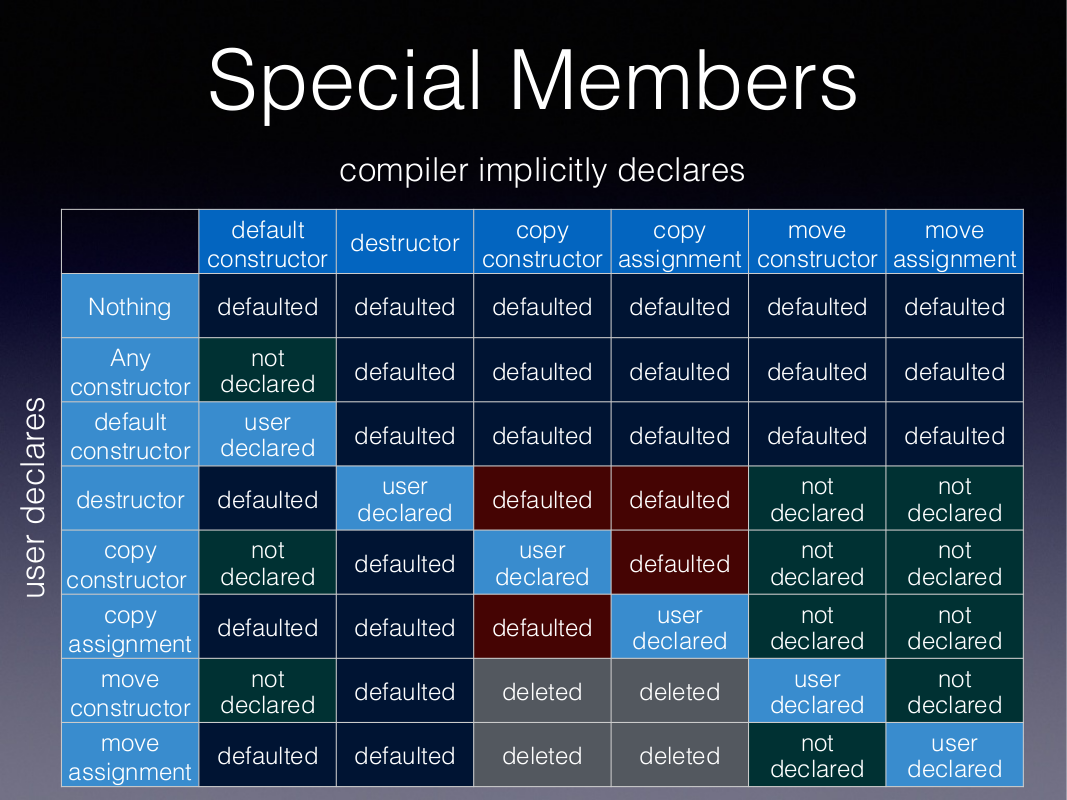
\includegraphics[width=1\textwidth, height=1\textheight, keepaspectratio]{./imgs/rule_of_five.png}
	\caption{Rule of Five}
	\label{fig:rule_of_five}
\end{figure}

%TODO: codice

%TODO: explicit keyword?

% -------------------------- SECTION: MOVE SEMANTICS ---------------------------------

\section{Move Semantics}

\textsf{\small \textbf{Definizione: } Le \textbf{move semantics} permettono, sotto certe condizioni, di trasferire la proprietà delle risorse esterne di qualche oggetto. Questo è importante per due motivi: } \\

\begin{enumerate}
	\item \textsf{\small Trasformare delle costose copie in delle move economiche.}
	\item \textsf{\small Implementare dei tipi di "move-only" sicure; ovvero tipi che per le copie non hanno senso, ma hanno senso per le move.}
	%\item \textsf{\small }
\end{enumerate}

\textsf{\small Per queste è molto importante il concetto di \textbf{lvalue} e di \textbf{rvalue}: } \\

\begin{itemize}
	\item \textsf{\small \textbf{lvalue T\&} : riguardano il copiare.}
	\item \textsf{\small \textbf{rvalue T\&\&} : riguardano il trasferire.}
\end{itemize}

\textsf{\small Per muovere un oggetto useremo \textbf{std::move(oggetto)}. Questa funzione restituisce un \textbf{rvalue} all'oggetto, così che possiamo rubare i dati dall'oggetto in quello nuovo.} \\

\textsf{\small \textbf{std::move(obj)} non cambia il contenuto dell'oggetto, ma \textbf{auto obj2 = std::move(obj)} possibilmente sì.} \\

\subsection{Fallbacks of move semantics}

\begin{enumerate}
	\item \textsf{\small Chiamare la \textbf{std::move()} su un oggetto costante, di solito, non produce effetti.}
	\begin{enumerate}
		\item \textsf{\small Non ha senso rimuovere o muovere/trasferire le risorse di un oggetto costante.}
		%\item \textsf{\small }
	\end{enumerate}
	\item \textsf{\small La semantica della copiatura è un ripiego soltanto se la semantica della copiatura è supportata.}
	\item \textsf{\small Se non c'è implementazione che prenda l'\textbf{rvalue} come argomento allora ci sarà l'ordinario e costante \textbf{lvalue} che verrà usato.}
	\item \textsf{\small Se una funzione non prende un \textbf{rvalue} e \textbf{lvalue} allora un errore a compile-time verrà generato.}
	\item \textsf{\small }
\end{enumerate}

\subsection{syntax vs semantics}

\textsf{\small \textbf{Syntax (Sintassi)}: } \\

\begin{itemize}
	\item \textsf{\small Riguarda le regole per scrivere qualsiasi cosa in un linguaggio di programmazione.}
	\item \textsf{\small Non ha niente a che fare con il significato di ciò che si è scritto.}
	\item \textsf{\small Una dichiarazione è sintatticamente valida se segue tutte le regole.}
	\item \textsf{\small È legata alla grammatica e alla struttura della lingua.}
	\item \textsf{\small Gli errori di sintassi si trovano dopo che il programma è stato eseguito.}
	\item \textsf{\small Alcuni esempi: un punto e virgola mancante. Sono errori semplice da trovare.}
\end{itemize}

\textsf{\small \textbf{Semantics (Semantica)}: } \\

\begin{itemize}
	\item \textsf{\small Riguarda il significato associato alla dichiarazione in una lingua di programmazione.}
	\item \textsf{\small È tutto riguardante il significato della dichiarazione che interpreta il programma.}
	\item \textsf{\small Gli errori sono gestiti a runtime.}
	\item \textsf{\small Si riferisce al significato delle linee di codice associate al linguaggio.}
	\item \textsf{\small Anche se un pezzo di codice ha la sintassi corretta, potrebbe comunque non fare ciò che voleva che facesse. Sono errori un po' più complicati da trovare.}
\end{itemize}

\begin{lstlisting}
	// Codice per dimostrare un errore semantico
	#include <iostream>
	
	int main()
	{
		// Dichiarazione di ritorno prima del cout
		return 0;
		
		std::cout << "Hello World!" << std::endl; // Output: nessun output perché è dopo il return statement.
	}
\end{lstlisting}

\begin{tabular}{|c|c|}
	\hline
	\textbf{Sintassi} & \textbf{Semantica} \\
	\hline
	\textsf{\small Si riferisce alle regole di } & \textsf{\small Si riferisce al significato associato } \\
	\textsf{\small qualsiasi riga di codice.} & \textsf{\small a qualsiasi riga di codice.} \\
	\hline
	\textsf{\small Errori di sintassi. Occorrono a compile time} & \textsf{\small Si riferisce ad un errore semantico. } \\
	\textsf{\small Alcuni esempi: } & \textsf{\small Occorre quando delle righe di codice } \\
	\textsf{\small mancanza di un punto e virgola.} & \textsf{\small sono valide sintatticamente,} \\
	\textsf{\small } & \textsf{\small ma non fanno quello che } \\
	\textsf{\small } & \textsf{\small il programmatore volesse che facessero.} \\
	\hline
\end{tabular}

\subsubsection{Ricapitolando le Move Semantics}

\textsf{\small Ricapitolando: } \\

\begin{itemize}
	\item \textsf{\small Le \textbf{Move Semantics} ci permettono di ottimizzare la copiatura di oggetti. È usato spesso implicitamente (per gli oggetti temporanei) o esplicitamente con \textbf{std::move()}.}
	\item \textsf{\small \textbf{std::move()} significa \emph{non ho più bisogno di questo valore}.}
	\item \textsf{\small Un oggetto segnato con \textbf{std::move()} non è mai parzialmente distrutto. Il distruttore verrà chiamato per distruggere l'oggetto appropriatamente.}
\end{itemize}

% -------------------------- SECTION: CLASSI ASTRATTE --------------------------------

\newpage

%TODO: abstract
%TODO: Pure Virtual

\section{Classi Astratte}

\textsf{\small \textbf{Definizione: } Una \textbf{classe astratta} è una classe generica dove non siamo in grado di implementare tutte le funzioni e che il suo unico scopo è quello di essere ereditata da altre classe che implementeranno le sue funzioni.} \\

\textsf{\small Una classe \textbf{astratta} per essere ritenuta tale deve, almeno, implementare una \textbf{pure virtual function}.} \\

\subsection{Pure Virtual Functions}

\textsf{\small \textbf{Definizione: } Una \textbf{pure virtual function} o \textbf{abstract function} è una funzione virtuale per cui non abbiamo bisogno di scrivere l'implementazione. Le implementazioni verranno poi implementate nelle classe derivate.} \\

\textsf{\small Si dichiara una \textbf{pure virtual function} assegnando 0 alla dichiarazione.} \\

\begin{lstlisting}
	class Test {
		public:
			// Pure Virtual Function
			virtual void show() = 0;
	};
\end{lstlisting}

\subsection{Abstract Class}

\textsf{\small \textbf{Definizione: } Proprietà di una \textbf{classe astratta}: } \\

\begin{itemize}
	\item \textsf{\small Possono avere funzioni normali e allo stesso tempo \textbf{pure virtual functions}.}
	\item \textsf{\small Non può essere instanziata, ma si possono creare puntatori e referenze della classe astratta.}
	\item \textsf{\small Le classi astratte sono usate principalmente per \textbf{Upcasting} così che la classe derivata possa usare la sua interfaccia.}
	\item \textsf{\small Se una \textbf{classe astratta} ha una classe derivata, essa deve implementare tutte le \textbf{pure virtual functions} altrimenti diventeranno anch'essi una classe \textbf{astratta}.}
	\item \textsf{\small }
	\item \textsf{\small }
\end{itemize}

\begin{lstlisting}
	#include <iostream>
	
	class Shape {
		public:
			virtual int getArea() = 0;
			void setWidth(int w)
			{
				width = w;
			}
		
			void setHeight(int h)
			{
				height = h;
			}
		
		protected:
			int width;
			int height;
			
	};

	class Rectangle : public Shape {
		public:
			int getArea()
			{
				return width * height;
			}
	};

	class Triangle : public Shape {
		public:
			int getArea()
			{
				return (width * height) / 2;
			}
	};

	int main()
	{
		Rectangle rect;
		Triangle tri;
		
		rect.setWidth(5);
		rect.setHeight(4);
		
		std::cout << "Area rettangolo: " << rect.getArea() << std::endl; // Output: Area Rettangolo: 20
		
		tri.setWidth(5);
		tri.setHeight(4);
		
		std::cout << "Area triangolo: " << tri.getArea() << std::endl; // Output: Area Triangolo: 10
		return 0;
	}
\end{lstlisting}

\subsection{Abstract class vs Interface}

\textsf{\small In un certo senso, possono quasi essere definite come, quelle che in altri linguaggi, si chiamano \textbf{Interfacce}, ovvero un'interfaccia mette semplicemente a disposizione le funzioni, ovvero le loro dichiarazioni e lascia a chi \textbf{implementa} l'interfaccia implementare queste funzioni. Il C++ non ha \textbf{Interfacce}, ma possiamo quasi dire che le \textbf{classi astratte} sono le \textbf{interfacce} del C++.} \break

\textsf{\small Quindi si può simulare un'interfaccia in C++ ponendo tutte le funzioni della classe \textbf{astratta} come \textbf{pure virtual functions}.} \\

% -------------------------- SECTION: ECCEZIONI --------------------------------------

%TODO: try/catch
%TODO: Errori a compile-time ed errori a runtime.
%TODO: throw.
%TODO: std::throw exception

\newpage

\section{Eccezioni}

\textsf{\small \textbf{Definizione: } Cosa sono le \textbf{eccezioni} (in inglese \emph{exceptions})? Le \textbf{eccezioni} sono delle anomalie o condizioni anormali incontrate durante l'esecuzione del programma.} \\

\textsf{\small Il C++ a differenza del C mette a disposizione delle keywords per occuparsi del codice che potrebbe lanciare un'eccezione.} \break

\textsf{\small Durante l'esecuzione del codice diversi errori potrebbero capitare: } \\

\begin{itemize}
	\item \textsf{\small errori nel codice.}
	\item \textsf{\small errori nell'input.}
	\item \textsf{\small altri tipi di errori.}
\end{itemize}

\textsf{\small Quando un errore occorre, C++, di solito, si fermerà e genererà un errore (lancerà un'eccezione).} \\

\subsection{try|catch|throw}

\textsf{\small \textbf{try, catch, throw}: Queste sono le keywords per \emph{Exception Handling} (Gestione delle eccezioni):}

\subsubsection{try}

\textsf{\small Il \textbf{try} ti permette di definire una porzione di codice che verrà testata durante la sua esecuzione. Ovvero se il blocco di codice nel try non lancerà alcuna eccezione allora verrà eseguito il try e poi il codice seguente ad esso, altrimenti verrà eseguito il codice nella clausola \textbf{catch}.} \\

\subsubsection{catch}

\textsf{\small Il \textbf{catch} ti permette di definire un blocco di codice che verrà eseguito se un errore sarà accorso nel \textbf{try}.} \\

\begin{lstlisting}
	try {
		// Blocco di codice del try.
	}catch(NomeEccezione e){
		// Blocco di codice del catch.
	}
\end{lstlisting}

\textsf{\small C'è uno special catch chiamato \emph{catch all} che permette di "catturare" tutte le eccezioni. Si fa in questo modo: \textbf{catch(...) (quindi un catch con l'ellissi, ovvero i tre puntini).}}

\subsubsection{std::throw exception}

\textsf{\small Il \textbf{throw} ti permette di lanciare un'eccezione quando un problema è stato rilevato.} \\

\begin{lstlisting}
	double division(int a, int b)
	{
		if(b == 0)
		{
			std::throw "Divisione per zero!";
		}
		return a/b;
	}

	int main()
	{
		int x = 22;
		int y = 0;
		double z = 0;
		
		try {
			z = division(x,y);
		}catch(const char* msg){
			//std::cerr è lo standard error, lo si può usare per mostrare errori sullo schermo.
			std::cerr << msg << std::endl; //Output: Divisione per zero!
		}
	
		return 0;
	}
\end{lstlisting}

\subsection{Errori a compile time ed errori a runtime}

\textsf{\small Gli errori a \textbf{compile time} sono degli errori che occorrono quando si violano le regole di sintassi del linguaggio, come per esempio: } \\

\begin{itemize}
	\item \textsf{\small Mancanza di una parentesi.}
	\item \textsf{\small Stampare il valore di una variabile senza dichiararla.}
	\item \textsf{\small Mancanza di un punto e virgola.}
\end{itemize}

\textsf{\small Gli errori a \textbf{runtime} sono quegli errori che occorrono durante l'esecuzione del programma dopo che la compilazione sia avvenuta con successo.} \break

\begin{tabular}{|c|c|}
	\hline
	\textbf{Compile-Time Errors} & \textbf{Runtime-Errors} \\
	\hline
	\textsf{\small Errori di sintassi.} & \textsf{\small Non sono rilevati dal compilatore.} \\
	\textsf{\small Prevengono l'esecuzione del codice.} & \textsf{\small Prevengono il codice dalla completa esecuzione.} \\
	\textsf{\small Vengono rilevati dal compilatore } & \textsf{\small Vengono fixati (sistemati) solo dopo} \\
	\textsf{\small e possono essere corretti} & \textsf{\small che il codice viene} \\
	\textsf{\small nel momento della programmazione.} & \textsf{\small eseguito.} \\
	\hline
\end{tabular}

%TODO: Volendo aggiungere immagine "exceptions_recap".
\subsection{Assertions}

\textsf{\small \textbf{Definizione: } Le \textbf{assertions} sono delle dichiarazioni usate per testare delle assunzioni fatte dal programmatore.} \\

\textsf{\small Se la condizione nell'\textbf{assert} fosse valutata falsa, allora il programma fermerebbe l'esecuzione.} \\

\begin{lstlisting}
	#include <assert.h>
	
	int length = 7;
	
	// Un assert per controllare che la variabile length sia maggiore o uguale a 0.
	assert(length >= 0);
	
	// Se l'assert fosse valutato 'false' il programma si fermerebbe e verrebbe mostrato quel messaggio.
	assert(length >= 0 && "La lunghezza non puo' essere negativa");
	
	int x = 0;
	
	// In questo caso verrebbe fermato il programma e verrebbe mostrato il messaggio "x deve essere maggiore di 0"
	assert(x > 0 && "x deve essere maggiore di 0"); 
\end{lstlisting}

% -------------------------- SECTION: OPERAZIONI DI I/O ------------------------------

\newpage

\section{Operazioni di Input/Output}

\textsf{\small \textbf{Definizione: } La libreria standard del C++ mette a disposizioni diverse funzioni per le operazioni di input ed output di dati in streams (flussi di dati), in files, ecc...} \\

\subsection{Input-Output stream}

\textsf{\small \textbf{Definizione: } Le \textbf{stream} sono sequenze, flussi di dati. Quando i dati provengono da dispositivi come tastiere, hard disk, connessioni network sono delle operazioni di \textbf{input}. Quando, invece i dati provengono da dispositivi come schermi, stampanti, disco rigido o una connessione network sono chiamati operazioni di \textbf{output}.} \break

\textsf{\small Il file di intestazione \textbf{<iostream>} definisce le funzioni come \textbf{cin, cout, cerr e clog} che corrispondono allo \emph{standard input}, \emph{standard output}, \emph{un-buffered standard error} e \emph{buffered standard error stream}.} \\

\textsf{\small Per quanto riguarda lo \emph{standard output} i dati vengono inseriti in esso attraverso l'operatore d'inserimento \textbf{<<}.} \break

\textsf{\small È possibile fare questo \emph{chaining} di \textbf{<<} perché l'operatore d'inserzione ritorna una referenza a cout (cout\&).} \\

\begin{lstlisting}
	#include <iostream>
	
	int main()
	{
		int x = 5;
		int y = 8;
		std::cout << "Valore di x: " << x << ", valore di y: " << y << std::endl; // Output: Valore di x: 5, valore di y: 8
		return 0;
	}
\end{lstlisting}

\textsf{\small Tramite \textbf{cin} chiediamo l'input dall'utente. In questa caso usiamo l'operatore di estrazione \textbf{>>}.} \\

\begin{lstlisting}
	#include <iostream>
	
	int main()
	{
		int age;
		
		std::cout << "Inserisci l'età: ";
		std::cin >> age;
		std::cout << "\n La tua età è: " << age << std::endl;
		return 0;
	}
\end{lstlisting}

\textsf{\small \textbf{cerr} è usato per mostrare degli errori sullo schermo. Un-buffered vuol dire che il messaggio non può essere immagazzinato, viene immediatamente mostrato sullo schermo.} \\

\begin{lstlisting}
	#include <iostream>
	
	int main()
	{
		std::cerr << "Si è verificato un errore!";
		return 0;
	}
\end{lstlisting}

\textsf{\small Anche \textbf{clog} come \textbf{cerr} mostra un errore, ma prima lo immagazzina all'interno di un buffer finché non è pieno o viene liberato (usando flush()) e poi verrà mostrato sullo schermo.} \\

\begin{lstlisting}
	#include <iostream>
	
	int main()
	{
		std::clog << "Si è verificato un errore";
		return 0;
	}
\end{lstlisting}

\subsubsection{std::endl vs newline}

\textsf{\small Qual è la differenza tra \textbf{std::endl} ed il carattere di escape newline \textbf{$\backslash$n}?} \\

\textsf{\small \textbf{$\backslash$n} va a capo, mentre \textbf{std::endl} va anch'esso a capo, ma in più ripulisce il buffer, di solito non hai sempre bisogno di farlo e questo ti costerà in termini di \emph{performance}.} \break

\begin{lstlisting}
	#include <iostream>
	
	std::cout << std::endl;
	// std::cout << std::endl è equivalente a:
	std::cout << '\n' << std::flush;
	// Mentre "$\backslash$n" inserisce semplicemente una nuova riga.
	std::cout << "\n";
\end{lstlisting} 

\begin{tabular}{|c|c|}
	\hline
	\textbf{std::endl} & \textbf{\small $\backslash$n} \\
	\hline
	\textsf{\small È un manipolatore.} & \textsf{\small È un carattere.} \\
	\hline
	\textsf{\small Non occupa spazio in memoria.} & \textsf{\small Occupa un byte visto che è un carattere.} \\
	\hline
	\textsf{\small È una keyword e non ha significato } & \textsf{\small Può essere memorizzata } \\
	\textsf{\small se la si memorizza in una stringa.} & \textsf{\small in una stringa e conserva il suo significato.} \\
	\hline
	\textsf{\small Non possiamo scrivere 'endl' in apici.} & \textsf{\small Possiamo scrivere sia '$\backslash$n' sia "$\backslash$n".} \\
	\hline
	\textsf{\small È supportata solo in C++.} & \textsf{\small È supportata sia in C che in C++.} \\
	\hline
	\textsf{\small Continua a ripulire il buffer.} & \textsf{\small Ripulisce il buffer solo alla fine del programma.} \\
	%\textsf{\small } & \textsf{\small } \\
	\hline
\end{tabular}

\textsf{\small Quindi, in conclusione, usare \textbf{$\backslash$n} sembra migliore in termini di prestazioni rispetto \textbf{std::endl} a meno che non sia necessario ripulire il buffer dello stream.} \break

\subsection{Manipolazione degli stream}

%TODO: <iomanip>

\textsf{\small \textbf{Definizione: } I \textbf{manipolatori} sono funzioni che permettono di manipolare \textbf{l'input/output} dello stream. Non vuol dire che modifichiamo la variabile, modifica soltanto lo stream.} \\

\textsf{\small Ci sono diversi tipi di manipolatori: } \\

\begin{enumerate}
	\item \textsf{\small \textbf{Manipolatori senza argomenti}: }
	\begin{itemize}
		\item \textsf{\small \textbf{endl} : serve per andare a capo e dopo averlo fatto ripulisce il buffer dello stream.}
		\item \textsf{\small \textbf{ws} : definito nell'\textbf{istream} e usato per ignorare gli spazi bianchi nella stringa dello stream.}
		\item \textsf{\small \textbf{ends} : inserisce un \emph{null character} nello stream.}
		\item \textsf{\small \textbf{flush} : definito nell'\textbf{ostream} e serve per ripulire l'output stream.}
	\end{itemize}
\end{enumerate}

\begin{lstlisting}
	#include <iostream>
	#include <istream>
	#include <sstream>
	#include <string>
	
	int main()
	{
		// istringstream da <sstream>
		std::istringstream str("   Hello World!");
		
		std::string line;
		
		// Ignora tutti gli spazi bianchi (con std::ws) prima della prima parola.
		std::getline( str >> std::ws, line);
		
		std::cout << line << std::endl;
		
		std::cout << "Test" << std::flush;
		
		std::cout << "A" << "\n";
		std::cout << "B" << std::ends;
		std::cout << "C" << std::endl;
		return 0;
	}
\end{lstlisting}

\begin{enumerate}
	\item \textsf{\small \textbf{Manipolatori con argomenti}: }
	\begin{enumerate}
		\item \textsf{\small \textbf{Alcuni importanti manipolatori in <iomanip>}: }
	\end{enumerate}
		\begin{itemize}
			\item \textsf{\small \textbf{setw(val)} : usato per impostare la larghezza dello spazio negli operatori di output.}
			\item \textsf{\small \textbf{setfill(c)} : usato per riempire lo stream di output con il carattere 'c'.}
			\item \textsf{\small \textbf{setprecision(val)} : Imposta val come nuovo valore di precisione dei valori floating-point.}
			\item \textsf{\small \textbf{setbase(val)} : Per impostare la base dei valori numerici. (es: base 2 (binario), base 16, esadecimale, base 8, ottale, ecc...)}
			\item \textsf{\small \textbf{setioflags(flag)} : Usato per impostare i flag di formato specificati dal parametro di maschera.}
			\item \textsf{\small \textbf{resetiosflags(m)} : Usato per resettare i flags di formato specificati dal parametro di maschera.}
		\end{itemize}
	\begin{enumerate}
		\item[b)] \textsf{\small \textbf{Alcuni manipolatori in <ios>} : }
	\end{enumerate}
		\begin{itemize}
			\item \textsf{\small \textbf{showpos} : Mostra il segno + nei numeri positivi.}
			\item \textsf{\small \textbf{noshowpos} : Non mostra il segno + nei numeri positivi.}
			\item \textsf{\small \textbf{showbase} : Indica la base numerica usati per i valori numerici.}
			\item \textsf{\small \textbf{uppercase} : Mostra le lettere in maiuscolo.}
			\item \textsf{\small \textbf{nouppercase} : Mostra le lettere in minuscolo.}
			\item \textsf{\small \textbf{fixed} : Usa la notazione decimale per i valori floating-point.}
			\item \textsf{\small \textbf{scientific} : Usa la notazione scientifica per i numeri in virgola mobile (floating-point).}
			\item \textsf{\small \textbf{hex} : Legge e scrive valori in esadecimale per i numeri interi e funziona come \emph{setbase(16)}.}
			\item \textsf{\small \textbf{dec} : Legge e scrive valori in decimale per i numeri interi, funziona come \emph{setbase(10)}.}
			\item \textsf{\small \textbf{oct} : Legge e scrive i valori in ottale per i numeri interi, funziona come \emph{setbase(8)}.}
			\item \textsf{\small \textbf{left} : Aggiusta l'output verso sinistra.}
			\item \textsf{\small \textbf{right} : Aggiusta l'output verso destra.}
			%\item \textsf{\small \textbf{} : }
		\end{itemize}
\end{enumerate}

\begin{lstlisting}
	#include <iostream>
	#include <iomanip>
	
	int main()
	{
		int a = 100;
		// Imposto la formattazione.
		std::cout << std::hex << std::left << std::showbase << std::nouppercase;
		
		std::cout << a << std::endl; // Output: 0x64 (esadecimale per 100)
		
		double b = 2001.5251;
		
		// Imposto la formattazione dello stream.
		std::cout << std::setbase(10) << std::right << std::setw(15)
		<< std::setfill('_') << std::showpos
		<< std::fixed << std::setprecision(2);
		
		// Mostro la variabile b
		std::cout << b << std::endl; // Output: \_\_\_\_\_\_\_+2001.53
		
		// Formattazione.
		std::cout << std::scientific << std::uppercase
		<< std::noshowpos << std::setprecision(9);
		
		double c = 201455.2646;
		
		// Stampo la variabile c.
		std::cout << c << std::endl; // Output: 2.014552646E+05
		
		return 0;
	}
\end{lstlisting}

\begin{figure}[ht]
	\centering
	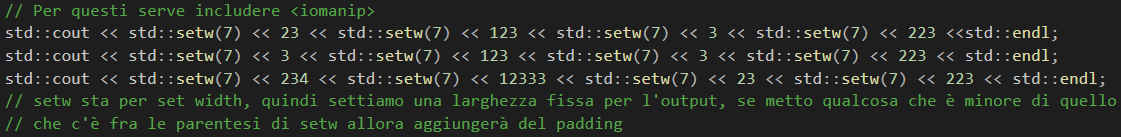
\includegraphics[width=1.2\textwidth, height=1.2\textheight, keepaspectratio]{./imgs/Stream_iomanip_setw.png}
	\caption{Stream iomanip}
	\label{fig:Stream_iomanip_setw}
\end{figure}

\subsection{Operazioni su file}

\textsf{\small \textbf{Definizione: } Per le operazioni di Input/Output sui files avremo bisogno di includere \textbf{fstream}.} \\

\textsf{\small Ci sono diverse modalità di apertura di un file: } \\

\begin{tabular}{|c|c|c|}
	\hline
	\textbf{Costante membra} & \textbf{Significato} & \textbf{Accesso} \\
	\hline
	\textsf{\small \textbf{in*}} & \textsf{\small input} & \textsf{\small File aperto per la lettura: } \\
	\textsf{\small \textbf{}} & \textsf{\small } & \textsf{\small il buffer interno supporta } \\
	\textsf{\small \textbf{}} & \textsf{\small } & \textsf{\small le operazioni di input.} \\
	\hline
	\textsf{\small \textbf{out}} & \textsf{\small output} & \textsf{\small File aperto per la scrittura.} \\
	\hline
	\textsf{\small \textbf{binary}} & \textsf{\small binary} & \textsf{\small Le operazioni vengono eseguite} \\
	\hline
	\textsf{\small \textbf{ate}} & \textsf{\small at end} & \textsf{\small La posizione di output parte dalla fine.} \\
	\hline
	\textsf{\small \textbf{app}} & \textsf{\small append} & \textsf{\small Parte dalla fine e aggiunge contenuti } \\
	\textsf{\small \textbf{}} & \textsf{\small } & \textsf{\small a quelli già presenti.} \\
	\hline
	\textsf{\small \textbf{trunc}} & \textsf{\small truncate} & \textsf{\small Tutti i contenuti } \\
	\textsf{\small \textbf{}} & \textsf{\small } & \textsf{\small che esistevano prima } \\
	\textsf{\small \textbf{}} & \textsf{\small } & \textsf{\small di essere aperto vengono scartati.} \\
	\hline
\end{tabular} \break

\textsf{\small Modalità di apertura di default: } \\

\begin{tabular}{|c|c|}
	\hline
	\textbf{Modalità di apertura di default} & \textbf{} \\
	\hline
	\textsf{\small ifstream} & \textsf{\small ios::in} \\
	\textsf{\small ofstream} & \textsf{\small ios::out} \\
	\textsf{\small fstream} & \textsf{\small ios::in | ios::out} \\
	\hline
\end{tabular}

\begin{lstlisting}
	// Esempio 1
	#include <iostream>
	#include <fstream>
	
	int main()
	{
		std::ofstream myfile;
		myfile.open("nomefile.txt");
		myfile << "Scrivere questa stringa nel file.\n";
		myfile.close();
		return 0;
	}
\end{lstlisting}

\begin{lstlisting}
	// Esempio 2
	#include <iostream>
	#include <fstream>
	
	int main()
	{
		std::string line;
		std::ifstream myfile("nomefile.txt");
		
		if(myfile.is_open())
		{
			while(std::getline(myfile, line))
			{
				std::cout << line << '\n';
			}
		myfile.close();
		} else {
			std::cout << "Impossibile aprire il file" << '\n';
		}
		return 0;
	}
\end{lstlisting}

\textsf{\small P.S. Ricordatevi di chiudere il file una volta che avete finito di utilizzarlo.} \\

\textsf{\small Uno dei modi per ottenere lo spazio occupato da un file: } \\

\begin{figure}[ht]
	\centering
	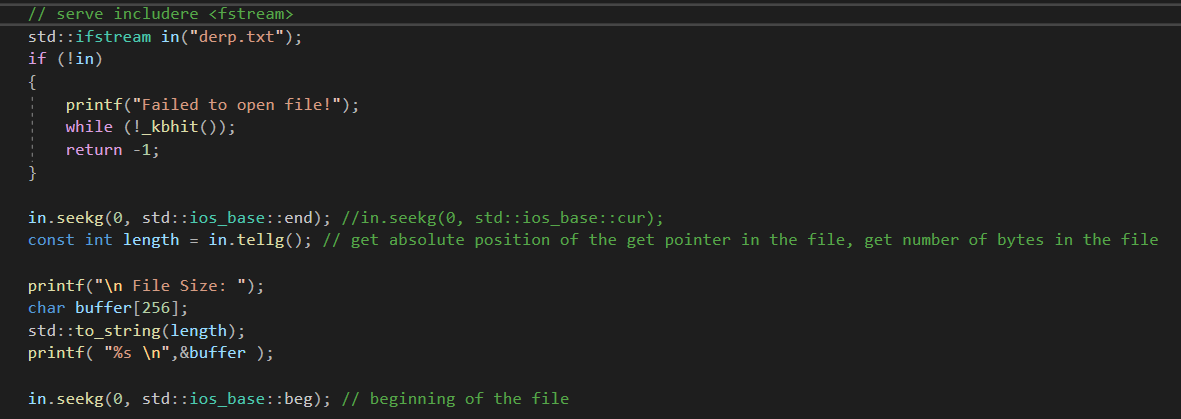
\includegraphics[width=1.2\textwidth, height=1.2\textheight, keepaspectratio]{./imgs/fstream_file_size.png}
	\caption{Ottenere il file size}
	\label{fig:fstream_file_size}
\end{figure}

\begin{figure}[ht]
	\centering
	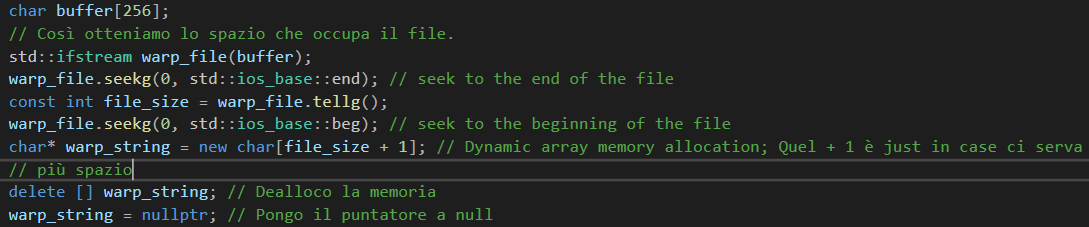
\includegraphics[width=1.2\textwidth, height=1.2\textheight, keepaspectratio]{./imgs/fstream_file_size2.png}
	\caption{Ottenere il file size}
	\label{fig:fstream_file_size2}
\end{figure}

% -------------------------- SECTION: STD::CHRONO ------------------------------------

\newpage

\section{std::chrono}

\textsf{\small \textbf{Definizione: } La libreria \textbf{chrono} è usata per occuparsi delle date e del tempo. Questa libreria è progettata col fatto che i timers e gli orologi potrebbero essere diversi su sistemi operativi differenti.} \\

\textsf{\small Fornisce una \emph{precisione neutrale}, attraverso la separazione le durate e il tempo.} \\

\textsf{\small Tutti gli elementi di questo header non sono definiti sotto il namespace std, ma sotto il \textbf{std::chrono namespace}.} \break

\textsf{\small Si occupa del tempo attraverso principalmente 3 concetti: } \\

\begin{itemize}
	\item \textsf{\small \textbf{Duration (Durata)} : Un oggetto durata esprime un intervallo di tempo come 3 minuti, 3 ore, 3 millisecondi, ecc.. Per esempio 33 secondi potrebbe essere rappresentato dalla durata di 33 ticks ciascuno di 1 secondo.}
	\item \textsf{\small \textbf{Clock (Orologio)} : Un orologio consiste in un punto di partenza (o epoch) e un tick rate.}
	\item \textsf{\small \textbf{Time point (Punto nel tempo)} : Un oggetto di tipo \emph{time\_point} esprime un punto nel tempo relativo ad un epoch di un clock. Internamente, l'oggetto memorizza un oggetto di tipo durata (\emph{duration}) e usa il clock come referenza per via del suo epoch.}
\end{itemize}

\subsection{Duration}

\begin{lstlisting}
	#include <iostream>
	#include <chrono>	
	
	int main ()
	{
		using namespace std::chrono;
		
		// std::chrono::milliseconds è una
		// instanzione di std::chrono::duration: - 1 secondo
		
		milliseconds mil(1000);
		
		mil = mil*60;
		
		std::cout << "durata (in periodi): ";
		std::cout << mil.count() << " millisecondi.\n"; // Output: durata (in periodi): 60000 millisecondi.
		
		std::cout << "durata (in secondi): ";
		std::cout << (mil.count() * milliseconds::period::num /
		milliseconds::period::den);
		std::cout << " secondi.\n"; // Output: durata (in secondi): 60 secondi.
		
		return 0;
	}
\end{lstlisting}

\subsection{Clock}

\textsf{\small Ci sono 3 diversi tipi di clock (orologi): } \\

\begin{itemize}
	\item \textsf{\small \textbf{system\_clock} : È il tempo corrente in base al sistema operativo (quello che vediamo nella barra dei comandi). È scritto come \emph{std::chrono::system\_clock}.}
	\item \textsf{\small \textbf{steady\_clock} : È un orologio monotonic (monotonico, uniforme) che non può essere aggiustato, regolato. Va ad un rate uniforme. È scritto come \emph{std::chrono::steady\_clock}.}
	\item \textsf{\small \textbf{high\_resolution\_clock} : Fornisce il periodo di tick più piccolo possibile. È scritto come \emph{std::chrono::high\_resolution\_clock}.}
\end{itemize}

\subsection{Time point}

\subsubsection{Calcolare il tempo di esecuzione di un blocco di codice}

\begin{lstlisting}
	// Esempio 1 Implementazione 1 per calcolare il tempo che un blocco di codice ci mette per essere eseguito.
	#include <iostream>
	#include <chrono>
	#include <ctime>
	
	long fibonacci(unsigned n)
	{
		if (n < 2) return n;
		return fibonacci(n-1) + fibonacci(n-2);
	}
	
	int main()
	{
		// time point e system\_clock
		std::chrono::time_point<std::chrono::system_clock> start, end;
		
		start = std::chrono::system_clock::now();
		std::cout << "f(42) = " << fibonacci(42) << '\n'; // Output: f(42) = 267914296
		end = std::chrono::system_clock::now();
		
		std::chrono::duration<double> elapsed_seconds = end - start;
		std::time_t end_time = std::chrono::system_clock::to_time_t(end);
		
		std::cout << "Finito di eseguire il " << std::ctime(&end_time)
		<< "tempo passato: " << elapsed_seconds.count() << "s\n"; // Output: Finito di eseguire il Sun Mar 13 22:53:59 2022 elapsed time: 2.71703s
	}
\end{lstlisting}

\textsf{\small Esempio 2 Implementazione 2 per calcolare il tempo di esecuzione di un blocco di codice: } \\

\begin{figure}[ht]
	\centering
	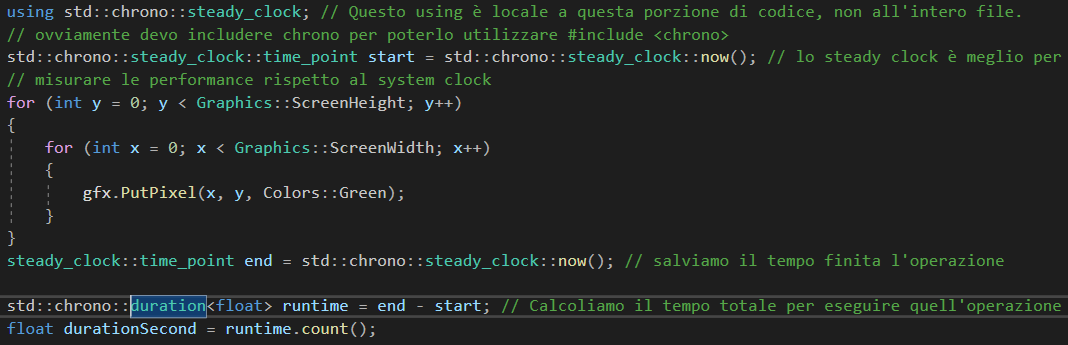
\includegraphics[width=1.2\textwidth, height=1.2\textheight, keepaspectratio]{./imgs/chrono_steady_clock_per_misurare_il_tempo_tra_una_operazione_e_l_altra_col_using.png}
	\caption{Calcolo tempo trascorso per eseguire un blocco di codice}
	\label{fig:chrono_steady_clock_per_misurare_il_tempo_tra_una_operazione_e_l_altra_col_using}
\end{figure}

% --------------------- SECTION: GENERATORI DI NUMERI CASUALI ------------------------

\newpage

\section{Generatori di numeri pseudo-casuali}

\textsf{\small \textbf{Definizione: } I \textbf{generatori di numeri pseudo-casuali} ci permettono di generare dei numeri che sembrano casuali. } \\

\subsection{Numeri casuali come in C}

\textsf{\small In C e di conseguenza in C++ si può utilizzare \textbf{rand()} e \textbf{srand()} importando \textbf{stdlib.h} in C e \textbf{<cstdlib>} in C++.} \\

\begin{lstlisting}
	// Esempio 1
	#include <iostream>
	#include <cstdlib>
	
	// Questo programma genererà sempre la stessa sequenza di numeri ad ogni esecuzione.
	int main()
	{
		int number;
		for(int i = 0; i < 3; i++)
		{
			number = rand();
			std::cout << number << std::endl;
		}
		return 0;
	}
\end{lstlisting}

\textsf{\small Per generare un numero compreso in un range (raggio: tra due numeri) usiamo l'operatore modulo e il numero a cui può arrivare.} \\

\begin{lstlisting}
	// Esempio 2
	#include <iostream>
	#include <cstdlib>
	
	// Questo programma genererà un numero nel range 25 e 50.
	int main()
	{
		int max = 50;
		int min = 25;
		int range = max - min + 1;
		
		int num = rand() % range + min;
		return 0;
	}
\end{lstlisting}

\textsf{\small \textbf{Definizione: } Il \textbf{seed} (seme) è il punto d'inizio della sequenza, può essere cambiato affinché la sequenza di numeri generati sia diversa.} \\

\textsf{\small Nel prossimo esempio usiamo il tempo corrente per generare un \emph{seed} (un seme). Usiamo \textbf{srand} per impostare il seme. } \\

\begin{lstlisting}
	// Esempio 3
	#include <iostream>
	#include <cstdlib>
	#include <time.h>
	
	// Questo programma genererà un numero nel range 25 e 50.
	int main()
	{
		
		constexpr int NUM_OF_NUMBERS = 3;
		
		int number;
		
		// Usiamo srand per settare il seed ed usiamo il tempo corrente in questo caso come parametro del seed.
		std::srand(time(0));
		
		for(int i = 0; i < NUM_OF_NUMBERS; i++)
		{
			number = rand();
			std::cout << number << std::endl;
		}
		return 0;
	}
\end{lstlisting}

\subsection{Cosa vuol dire e perché pseudo-random?}

\textsf{\small Gli \textbf{pseudorandom number generator} (\emph{PRNG}), anche chiamati \textbf{deterministic random bit generator} (\emph{DRBG}, ovvero generatori di bit casuali deterministici) sono degli algoritmi per generare sequenze di numeri le quali proprietà sono simili a quelle delle sequenze di numeri casuali.} \\

\textsf{\small I \emph{PRNG} non generano vere sequenze casuali perché è completamente determinato da un numero di partenza chiamato \emph{seed} (seme).} \break

\textsf{\small Quindi è chiamato "\emph{pseudo}" casuale perché l'algoritmo può ripetere la sequenza e quindi i numeri non sono propriamente casuali.} \\

\subsection{I vari tipi di generatori}

\textsf{\small \textbf{Definizione: } Nell'header \textbf{<random>} sono contenuti diversi generatori di numeri pseudo-casuali e diverse distribuzioni:} \\

\begin{itemize}
	\item \textsf{\small \textbf{Generatori} : oggetti che generano numeri distribuiti uniformemente.}
	\item \textsf{\small \textbf{Distribuzioni} : oggetti che trasformano sequenze di numeri generati da un generatore in sequenze di numeri che seguono una specifica distribuzione variabili e casuale, come: uniforme, normale, binomiale.}
\end{itemize}

\begin{enumerate}[I]
	\item \textsf{\small \textbf{Pseudo-random number engines} : usano un algoritmo per generare numeri casuali basati su un seme iniziale. Questi sono: }
\end{enumerate}

\begin{figure}[ht]
	\centering
	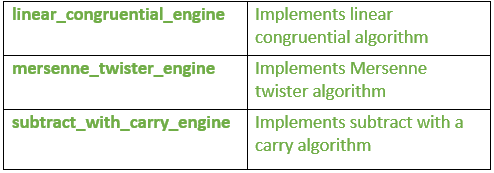
\includegraphics[width=1.2\textwidth, height=1.2\textheight, keepaspectratio]{./imgs/random-number-engines.png}
	\caption{Motori di numeri pseudo-casuali}
	\label{fig:random-number-engines}
\end{figure}

\begin{enumerate}
	\item \textsf{\small \textbf{linear\_congruential\_engine} : è il più semplice nella \textbf{STL} (\emph{Standard Template Library}) che genera numeri interi senza segno.}
\end{enumerate}

\begin{lstlisting}
	#include <iostream>
	#include <chrono>
	#include <random>
	
	int main()
	{
		// Trova il tempo tra il clock del sistema (tempo corrente) e l'epoch del clock (data e tempo relativi quando il timestamp di un clock di un computer sono determinati).
		unsigned seed = std::chrono::system_clock::now().time_since_epoch().count();
		
		std::minstd_rand0 generator(seed);
		
		std::cout << generator() << "è un numero casuale tra ";
		std::cout << generator.min() << " e " << generator.max();
		return 0;
	}
\end{lstlisting}

\begin{enumerate}
	\item[2.] \textsf{\small \textbf{mersenne\_twister\_engine} : È un motore di numeri casuali basati sull'algoritmo \emph{Mersenne Twister}. Produce dei numeri senza segno di alta qualità nell'intervallo [$0, (2^w)-1]$. dove \emph{w = size della parola (word)}.} \\
\end{enumerate}

\begin{lstlisting}
	// Esempio 1
	#include <iostream>
	#include <chrono>
	#include <random>
	
	int main()
	{
		unsigned seed = std::chrono::system_clock::now().time_since_epoch().count();
		
		std::mt19937 generator(seed);
		
		std::cout << generator() << " è un numero casuale tra ";
		
		std::cout << generator.min() << " e " << generator.max();
		return 0;
	}
\end{lstlisting}

\begin{lstlisting}
	// Esempio 2
	#include <iostream>
	#include <chrono>
	#include <random>
	
	int randomNumberGenerator(int limit)
	{
		// generatore di numeri interi casuali con distribuzione uniforme che produce numeri casuali non deterministici.
		std::random_device rd;
		
		// Generatore pseudo-random con l'algoritmo Mersenne Twister di numeri a 32 bit con uno spazio di stato di 19937 bits.
		std::mt19937 rng(rd());
		
		// Distribuzione uniforme
		std::uniform_int_distribution<> dis(1, limit);
		return dis(rng);
	}
	
	int main()
	{
		int limit = 100;
		std::cout << randomNumberGenerator(limit) << std::endl;
		return 0;
	}
\end{lstlisting}

\begin{enumerate}
	\item[3.] \textsf{\small \textbf{subtract\_with\_carry\_engine} : È un motore di generazione di numeri pseudo-casuali che produce numeri interi senza segno. L'algoritmo usato è il \emph{generatore di fibonacci} con una sequenza di stati di r elementi, più uno per il carry (il resto).} \\
\end{enumerate}

\begin{lstlisting}
	#include <iostream>
	#include <chrono>
	#include <random>
	
	int main()
	{
		unsigned seed = std::chrono::system_clock::now().time_since_epoch().count();
		
		std::subtract_with_carry_engine<unsigned, 24, 10, 24> generator(seed);
		
		std::cout << generator() << " è un numero casuale tra ";
		
		std::cout << generator.min() << " e " << generator.max();
		return 0;
	}
\end{lstlisting}

\begin{enumerate}[I]
	\item[II] \textsf{\small \textbf{Random number generator} : È un generatore di numeri casuali che produce numeri casuali non deterministici.} \\
\end{enumerate}

\begin{lstlisting}
	#include <iostream>
	#include <random>
	
	int main ()
	{
		std::random_device rd;
		
		std::cout << "default random_device caratteristiche:" << std::endl;
		
		std::cout << "minimo: " << rd.min() << std::endl;
		
		std::cout << "massimo: " << rd.max() << std::endl;
		
		std::cout << "entropia: " << rd.entropy() << std::endl;
		
		std::cout << "un numero casuale: " << rd() << std::endl;
		
		return 0;
	}
\end{lstlisting}

\begin{enumerate}[I]
	\item[III] \textsf{\small \textbf{Pseudo-random number engines (instantions)} : Questi sono particolari instanzioni di motori di generatori e adattatori: } \\
\end{enumerate}

\begin{figure}[ht]
	\centering
	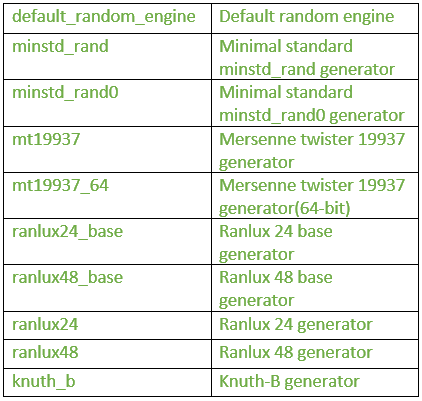
\includegraphics[width=1\textwidth, height=1\textheight, keepaspectratio]{./imgs/pseudo-random-number-engines.png}
	\caption{Motori di numeri pseudo casuali}
	\label{fig:pseudo-random-number-engines}
\end{figure}

\begin{enumerate}
	\item \textsf{\small \textbf{default\_random\_engine} : Questo è una classe che genera numeri pseudo-casuali.} \\
\end{enumerate}

\begin{lstlisting}
	#include <iostream>
	#include <chrono>
	#include <random>
	
	int main()
	{
		
		unsigned seed = std::chrono::system_clock::now().time_since_epoch().count();
		
		// minstd\_rand0 è un standard linear\_congruential\_engine
		std::minstd_rand0 generator(seed);
		
		std::cout << generator() << " è un numero casuale tra ";
		
		std::cout << generator.min() << " e " << generator.max();
		
		return 0;
	}
\end{lstlisting}

\begin{enumerate}
	\item[2.] \textsf{\small \textbf{minstd\_rand} : Genera numeri pseudo casuali. È simile al linear congruential generator.} \\
\end{enumerate}

\begin{lstlisting}
	#include <iostream>
	#include <chrono>
	#include <random>
	
	int main()
	{
		
		unsigned seed = chrono::system_clock::now().time_since_epoch().count();
		
		// minstd\_rand0 è un standard
		//linear\_congruential\_engine
		std::minstd_rand0 generator(seed);
		
		std::cout << generator() << " è un numero casuale tra ";
		
		std::cout << generator.min() << " e " << generator.max();
		
		return 0;
	}
\end{lstlisting}

\begin{enumerate}
	\item[3.] \textsf{\small \textbf{mt19937} : È il generatore \emph{Mersenne Twister} 19937. È un generatore di numeri a 32 bit con uno spazio di stato di 19937 bits.} \\
\end{enumerate}

\begin{enumerate}
	\item[4.] \textsf{\small \textbf{ranlux24\_base} : È un generatore \emph{Ranlux base 24}. È un generatore pseudo casuale che sottrae con il resto di numeri a 24-bit, generalmente usato come base per il generatore \emph{ranlux24}.} \\
\end{enumerate}

\begin{lstlisting}
	#include <iostream>
	#include <chrono>
	#include <random>
	
	int main ()
	{	
		unsigned seed = std::chrono::system_clock::now().time_since_epoch().count();
		std::subtract_with_carry_engine<unsigned,24,10,24> generator(seed);
		
		std::cout << generator() << " è un numero casuale tra ";
		
		std::cout << generator.min() << " e " << generator.max();
		
		return 0;
	}
\end{lstlisting}

\begin{enumerate}[I]
	\item[IV] \textsf{\small \textbf{Engine Adaptors}} \\
\end{enumerate}

\begin{enumerate}
	\item \textsf{\small \textbf{discard\_block\_engine} : È una classe template che adatta un motore di generatore di numeri pseudo-casuali attraverso il solo utilizzo di 'r' elementi di ogni blocco e 'p' elementi dalla sequenza che produce, scartando il resto. L'adattatore tiene un contatore interno per tenere traccia di quanti elementi sono stati prodotti nel blocco corrente.}
\end{enumerate}

\textsf{\small I generatori \textbf{ranlux24} e \textbf{ranlux48} adattano un \textbf{subtract\_with\_carry\_engine} usando questo adattatore.} \\

\begin{lstlisting}
	#include <iostream>
	#include <chrono>
	#include <random>
	
	int main ()
	{
		unsigned seed = std::chrono::system_clock::now().time_since_epoch().count();
		
		// ranlux24 è un standard instantitation
		// del discard\_block\_engine:
		std::ranlux24 generator(seed);
		
		std::cout << generator() << " è un numero casuale tra ";
		
		std::cout << generator.min() << " e " << generator.max();
		
		return 0;
	}
\end{lstlisting}

\begin{enumerate}
	\item[2.] \textsf{\small \textbf{indipendent\_bits\_engine} : È un adattatore che adatta un motore di generatore di numeri casuali per produrre numeri con uno specifico numero di bits (w).}
\end{enumerate}

\begin{lstlisting}
	#include <iostream>
	#include <chrono>
	#include <cstdint>
	#include <random>
	
	int main ()
	{
		unsigned seed = std::chrono::system_clock::now().time_since_epoch().count();
		
		// independent\_bits\_engine
		std::independent_bits_engine<mt19937,64,uint_fast64_t> generator(seed);
		
		std::cout << generator() << " è un numero casuale tra ";
		
		std::cout << generator.min() << " e " << generator.max();
		
		return 0;
	}
\end{lstlisting}

\begin{enumerate}
	\item[3.] \textsf{\small \textbf{shuffle\_order\_engine} : È un adattatore che adatta un motore di generatore di numeri pseudo-casuali così che i numeri siano ottenuti in una sequenza differente.}
\end{enumerate}

\textsf{\small L'oggetto mantiene un buffer di k numeri generati internamente e quando richiesti restituisce alcuni selezionati casualmente nel buffer, rimpiazzandolo con un valore ottenuto dalla base del motore.} \\

\begin{lstlisting}
	#include <iostream>
	#include <chrono>
	#include <random>
	
	int main ()
	{
		unsigned seed = std::chrono::system_clock::now().time_since_epoch().count();
		
		// ranlux24 è un standard instantitation
		// del discard\_block\_engine:
		ranlux24 generator (seed);
		
		std::cout << generator() << " è un numero casuale tra ";
		
		std::cout << generator.min() << " e " << generator.max();
		
		return 0;
	}
\end{lstlisting}

% ------------------------ SECTION: MAP, SET, PAIR, HASH -----------------------------

\newpage

\section{Map | Set | Pair | Hash}

\textsf{\small \textbf{Definizione: } } \\

%TODO: map, hashmap, set, pair

% -------------------------- SECTION: TYPE TRAITS ------------------------------------

\newpage

\section{Type Traits}

\textsf{\small \textbf{Definizione: } } \\

%TODO: include <type_traits>
%TODO: typeid
%TODO: decltype

% ------------------------------------------------------------------------------------

%TODO: C++20 oppure in un capitolo a parte?